\documentclass[12pt,oneside]{report}

\usepackage[letterpaper,margin=1in]{geometry}
\usepackage[T1]{fontenc}
\usepackage[utf8]{inputenc}
\usepackage{lmodern}
\usepackage{microtype}
\usepackage{setspace}
\usepackage{csquotes}
\usepackage{graphicx}
\usepackage{booktabs}
\usepackage{longtable}
\usepackage{tabularx}
\usepackage{array}
\usepackage{multirow}
\usepackage{amsmath,amssymb,amsthm,mathtools,bm}
\usepackage{siunitx}
\usepackage{float}
\usepackage{caption}
\usepackage{subcaption}
\usepackage{enumitem}
\usepackage{xcolor}
\usepackage{tikz}
\usetikzlibrary{arrows.meta,positioning,shapes.geometric,calc,fit}
\usepackage[hidelinks]{hyperref}
\usepackage[nameinlink,noabbrev]{cleveref}
\usepackage{pdflscape}
\usepackage{appendix}
\usepackage{fancyhdr}
\usepackage{titlesec}
\usepackage{listings}
\usepackage[backend=biber,style=numeric-comp,sorting=nyt,maxbibnames=99,giveninits=true]{biblatex}
\addbibresource{references.bib}

\sisetup{detect-all,separate-uncertainty=true,per-mode=symbol}
\setstretch{1.35}
\setlength{\parindent}{1.5em}
\setlength{\parskip}{0.25em}
\setcounter{secnumdepth}{3}
\setcounter{tocdepth}{2}
\graphicspath{{figures/}}

\setlength{\headheight}{15pt}
\pagestyle{fancy}
\fancyhf{}
\fancyhead[L]{\nouppercase{\leftmark}}
\fancyhead[R]{\thepage}
\renewcommand{\headrulewidth}{0.4pt}

\newcommand{\ThesisTitle}{Biological Implications of Suppressing Radiation Emissions from Relativistic Plasmas Using Magnetic Perturbations}
\newcommand{\ThesisSubtitle}{A Multiscale Framework for Source-Term Control, Dosimetry, and Radiobiological Risk}
\newcommand{\AuthorName}{Zachary R. Tullier}
\newcommand{\DegreeName}{Master of Science}
\newcommand{\CollegeName}{College of Science and Engineering}
\newcommand{\UniversityName}{University of Houston--Clear Lake}
\newcommand{\ThesisDate}{July 2026}

\newcommand{\Te}{T_{\mathrm e}}
\newcommand{\Ti}{T_{\mathrm i}}
\newcommand{\nelec}{n_{\mathrm e}}
\newcommand{\nion}{n_{\mathrm i}}
\newcommand{\Egamma}{E_{\gamma}}
\newcommand{\mecsq}{m_{\mathrm e}c^2}
\newcommand{\Zeff}{Z_{\mathrm{eff}}}
\newcommand{\dd}{\mathrm{d}}
\newcommand{\eV}{\mathrm{eV}}
\newcommand{\keV}{\mathrm{keV}}
\newcommand{\MeV}{\mathrm{MeV}}
\newcommand{\Gy}{\mathrm{Gy}}
\newcommand{\Sv}{\mathrm{Sv}}
\newcommand{\pB}{\ensuremath{p\text{--}{}^{11}\mathrm B}}

\theoremstyle{definition}
\newtheorem{definition}{Definition}[chapter]
\newtheorem{assumption}{Assumption}[chapter]
\newtheorem{proposition}{Proposition}[chapter]

\lstset{
  basicstyle=\ttfamily\small,
  frame=single,
  breaklines=true,
  columns=fullflexible,
  showstringspaces=false
}

\begin{document}

\begin{titlepage}
\centering
\vspace*{0.8in}
{\Large\bfseries \ThesisTitle\par}
\vspace{0.25in}
{\large \ThesisSubtitle\par}
\vspace{0.8in}
{\large A Thesis\par}
\vspace{0.2in}
{Presented to the Academic Faculty\par}
\vspace{0.6in}
{by\par}
\vspace{0.2in}
{\Large \AuthorName\par}
\vfill
{In Partial Fulfillment of the Requirements for the Degree of\par}
{\DegreeName\ in the \CollegeName\par}
\vspace{0.45in}
{\UniversityName\par}
{\ThesisDate\par}
\vspace{0.4in}
{Copyright \textcopyright\ \AuthorName\ 2026}
\end{titlepage}

\pagenumbering{roman}

\chapter*{Approval Page}
%% Define your committee members. If you have less than 6, simple delete/comment the unused lines
\newcommand*{\SignatureAndDate}[3]{
    \par\noindent\makebox[2.5in]{\hrulefill} \hfill\makebox[2.0in]{\hrulefill}
    \par\noindent\makebox[2.5in][l]{#1}      \hfill\makebox[2.0in][l]{Date}
    \par\noindent\makebox[2.5in][l]{#2}
    \par\noindent\makebox[2.5in][l]{#3}}

\SignatureAndDate{Samina S. Masood}{Ph.D., Chair}{Thesis Advisor}
\vspace{.2in}
\SignatureAndDate{Brandon Reddell}{Ph.D}{Thesis Committee}

\vspace{.3in}
\begin{center}
    {\fontfamily{qcr}\selectfont APPROVED BY THE COLLEGE OF SCIENCE AND ENGINEERING}
\end{center}

\SignatureAndDate{David Garrison}{Ph.D}{Associate Dean}
\vspace{.2in}
\SignatureAndDate{Jennifer Irvin}{Ph.D}{Dean}



\chapter*{Dedication}
\addcontentsline{toc}{chapter}{Dedication}
\begin{center}
\emph{This thesis is dedicated to my family, whose love, patience, and encouragement made this accomplishment possible.
To my father, whose questions continually challenged me to clarify my goals, refine my thinking, and find the path that was truly right for me. Your curiosity and guidance helped shape both my academic direction and the person I have become.
To my mother, whose insight and thoughtful questions pushed me to look beyond the technical details and consider the deeper value, purpose, and impact of research. You taught me that meaningful work should not only expand knowledge, but also serve a greater purpose.
To Erin, thank you for your unwavering support, patience, and belief in me throughout this journey. To Maci and Miley, you are my greatest inspiration and the reason I continue to strive for a better future.
This work is a reflection of the love, wisdom, and encouragement each of you has given me.
}
\end{center}
\clearpage

\chapter*{Acknowledgements}
\addcontentsline{toc}{chapter}{Acknowledgements}
I would like to express my sincere gratitude to my thesis advisor, Dr. Masood, for their guidance, patience, and continued support throughout the development of this research. Their insight and expertise were invaluable in shaping the direction of this thesis and strengthening my understanding of plasma physics, radiation processes, and scientific research.

I am grateful to the faculty and staff of the Department of Mathematical, Applied, and Physical Sciences at the University of Houston - Clear Lake for providing the educational foundation, resources, and opportunities necessary to complete this degree. I would also like to acknowledge the authors, researchers, and educators whose work in plasma physics, fusion science, radiation transport, and radiation biology provided the foundation for this interdisciplinary study.

Most importantly, I would like to thank my family for their unconditional love, patience, and encouragement. To my father, whose questions continually challenged me to clarify my goals, refine my thinking, and find the path that was truly right for me. Your curiosity and guidance helped shape both my academic direction and the person I have become. To my mother, whose insight and thoughtful questions pushed me to look beyond the technical details and consider the deeper value, purpose, and impact of research. You taught me that meaningful work should not only expand knowledge, but also serve a greater purpose. To Erin, thank you for standing beside me, believing in me, and supporting me throughout every stage of this journey. To Maci and Miley, you have been my greatest source of inspiration and motivation. This work is a reflection of the love, wisdom, and encouragement each of you has given me.

Finally, I am thankful for the perseverance, strength, and opportunities that allowed me to reach this milestone. This thesis represents not only an academic achievement, but also the support, sacrifice, and encouragement of everyone who helped me along the way.

\clearpage

\chapter*{Abstract}
\addcontentsline{toc}{chapter}{Abstract}
Relativistic plasmas can radiate a substantial fraction of their stored energy through electron--ion and electron--electron bremsstrahlung, synchrotron emission, and related high-energy photon processes. These losses are a central obstacle for advanced fusion fuels such as proton--boron-11, and the escaping photon field is also an external radiation source relevant to shielding, occupational exposure, instrumentation, and biological risk. This thesis develops a unified plasma-physics and radiation-biology framework for evaluating whether controlled magnetic perturbations can reduce both the radiative power loss inside a relativistic plasma and the biological burden outside it.

The central physical hypothesis is that magnetic perturbations, open-field-line transport, ambipolar potentials, resonant diffusion, and related distribution-function controls can selectively deplete or redistribute superthermal electrons. Because relativistic bremsstrahlung is disproportionately weighted toward the high-energy tail, a number-conserving redistribution of those electrons to lower energy can reduce total and spectrally resolved emission. The central biological hypothesis is that a reduction in emitted spectral energy fluence produces a calculable reduction in absorbed dose, DNA damage burden, clonogenic injury, and stochastic risk, but that the magnitude of the biological benefit depends on photon energy, geometry, attenuation, dose rate, and tissue response.

A multiscale model is formulated from the electron distribution function to bremsstrahlung emissivity, photon transport, absorbed dose, track structure, molecular damage, and cell survival. The thesis distinguishes source-term suppression from shielding and emphasizes that the two strategies are multiplicative rather than interchangeable. It also identifies conditions under which apparent radiative suppression could be offset by increased particle loss, synchrotron emission, spectral hardening, localized hot spots, or activation products. No unreported experimental data are asserted. Numerical examples are explicitly presented as reproducible, illustrative calculations whose purpose is to define the measurements and simulations required for a definitive validation campaign.

The resulting framework provides a defensible bridge between relativistic plasma engineering and radiobiology: magnetic control is evaluated not only by watts of radiative loss avoided, but also by spectral dose reduction and biologically weighted consequence. This approach is applicable to advanced-fuel fusion concepts, mirror and open-field-line systems, laser-produced plasmas, dense plasma focus devices, accelerator-driven plasma sources, and any environment in which plasma-generated ionizing radiation may reach workers, patients, electronics, or biological specimens.
\clearpage

\chapter*{Executive Summary}
\addcontentsline{toc}{chapter}{Executive Summary}
The original plasma problem is an energy-balance problem: energetic electrons collide with ions and other electrons, producing bremsstrahlung that removes useful plasma energy. In relativistic regimes, the high-energy tail of the electron distribution matters more than its small particle fraction might suggest. A magnetic configuration that preferentially removes, scatters, or decelerates those electrons can therefore change the radiation source at its origin. The radiation-biology extension asks a second question: what does that source change mean after the photons leave the plasma?

The answer requires five linked models. First, a kinetic model predicts the electron distribution under collisions, acceleration, magnetic perturbations, and losses. Second, differential electron--ion and electron--electron cross sections convert that distribution into a photon spectrum. Third, radiation-transport calculations propagate the spectrum through vacuum windows, structures, shielding, air, and tissue. Fourth, dosimetry converts energy fluence into absorbed dose. Fifth, radiobiological models translate dose and radiation quality into measurable endpoints such as DNA double-strand breaks, chromosome aberrations, surviving fraction, tissue reaction probability, or long-term risk.

The thesis makes four principal contributions. It defines a number-conserving cutoff-and-redistribution operator suitable for theoretical studies of superthermal-tail control. It shows how magnetic perturbation parameters enter an energy-dependent escape or diffusion term in a relativistic Fokker--Planck equation. It derives a source-to-dose response operator that preserves spectral information rather than equating all emitted watts. Finally, it establishes a validation plan in which plasma diagnostics, X-ray spectroscopy, Monte Carlo transport, physical dosimetry, and biological assays are performed on a shared configuration.

The most important conclusion is conceptual: a percentage reduction in total bremsstrahlung power is not automatically the same percentage reduction in biological effect. If suppression removes mainly low-energy photons, shielding and shallow tissue dose may improve strongly while deep dose changes less. If it removes mainly high-energy photons, penetrating dose and secondary-electron ranges may decrease disproportionately. Conversely, a harder residual spectrum could partly offset a reduction in integrated power at a distant location. Therefore, the correct optimization objective is a weighted spectral functional, not only total radiated power.
\clearpage

\tableofcontents
\listoftables
\listoffigures
\clearpage

\chapter*{Nomenclature}
\addcontentsline{toc}{chapter}{Nomenclature}
\begin{longtable}{p{0.22\textwidth}p{0.70\textwidth}}
$B_0$, $\delta B$ & Equilibrium and perturbing magnetic-field amplitudes \\
$D$ & Absorbed dose, joule per kilogram (gray) \\
$E$, $\Egamma$ & Electron kinetic energy and photon energy \\
$f(\mathbf{x},\mathbf{p},t)$ & Electron distribution function \\
$H_T$ & Equivalent dose to tissue or organ $T$ \\
$K_2$ & Modified Bessel function of the second kind \\
$L_c$ & Magnetic correlation length \\
$P_{\mathrm{Br}}$ & Bremsstrahlung power \\
$R_m$ & Magnetic mirror ratio \\
$S(D)$ & Clonogenic surviving fraction after absorbed dose $D$ \\
$\theta$ & Dimensionless electron temperature, $k_B\Te/(m_ec^2)$ \\
$\mu/\rho$ & Mass attenuation coefficient \\
$\mu_{\mathrm{en}}/\rho$ & Mass energy-absorption coefficient \\
$\Phi_E$ & Differential photon fluence \\
$\Zeff$ & Effective ion charge \\
LET & Linear energy transfer \\
RBE & Relative biological effectiveness \\
RMP & Resonant magnetic perturbation \\
DSB/SSB & DNA double-strand/single-strand break \\
\end{longtable}
\clearpage

\pagenumbering{arabic}

\chapter{Introduction and Research Rationale}
\label{ch:introduction}

\section{The coupled plasma and biological problem}

High-temperature plasmas are simultaneously energy-conversion media and radiation sources. The same electrons that sustain ionization, carry current, exchange energy with ions, and participate in collective dynamics also emit photons when accelerated by Coulomb fields or magnetic curvature. At low electron temperature, thermal electron--ion bremsstrahlung is often treated as a correction to collisional power balance. At relativistic temperature, the correction can become a governing term: electron--electron emission becomes non-negligible, synchrotron power rises rapidly with energy and magnetic field, and a small superthermal population can dominate a broad part of the photon spectrum \cite{bekefi1966,rybicki1979,blumenthal1970,haug1975,nozawa1998}.

For advanced fusion fuels, especially \pB, this radiative coupling is unusually severe. The reaction releases three energetic alpha particles and avoids the primary \SI{14.1}{\MeV} neutron channel of deuterium--tritium fusion, but the plasma conditions required for useful reactivity are much more demanding. Electrons heated to tens or hundreds of kiloelectronvolts can radiate enough bremsstrahlung to erase the fusion power margin predicted by simple thermal models \cite{rider1995,nevins2000,sikora2016,wurzel2022}. Alpha channeling, non-Maxwellian ion populations, revised nuclear data, and improved confinement concepts have renewed interest in \pB, yet all of these approaches remain constrained by electron energy flow and radiation loss \cite{fisch1992,hay2015,ochs2022,ochs2025constraints}.

The biological problem begins at the plasma boundary. Escaping X rays and gamma rays interact with vessel walls, diagnostics, shielding, air, and tissue by photoelectric absorption, Compton scattering, and pair production. The energy transferred to charged secondary particles becomes absorbed dose; its spatial clustering controls molecular damage and contributes to cell killing, tissue reactions, and stochastic cancer risk \cite{attix1986,turner2007,baatout2023,hall2018,goodhead1994}. A plasma-physics optimization that reports only the reduction in total radiated power is therefore incomplete whenever personnel, biological samples, patients, or nearby electronics are part of the system. The spectrum, directionality, pulse structure, and geometry determine whether a reduction in watts becomes a comparable reduction in gray or sievert.

This thesis links these domains through a source-to-consequence chain:
\begin{equation}
\boxed{
 f_e(\mathbf{x},\mathbf{p},t)
 \rightarrow j_\gamma(\Egamma,\Omega,\mathbf{x},t)
 \rightarrow \Phi_\gamma(\Egamma,\mathbf{r},t)
 \rightarrow D(\mathbf{r})
 \rightarrow \mathcal{B}[D,\Egamma,\dot D,\mathrm{LET},\mathrm{biology}]
 }
\label{eq:source-to-biology}
\end{equation}
where $f_e$ is the electron distribution, $j_\gamma$ is spectral-angular photon emissivity, $\Phi_\gamma$ is transported fluence, $D$ is absorbed dose, and $\mathcal{B}$ denotes a biological-response operator. The scientific bridge is not metaphorical. Each arrow corresponds to a measurable or computable transfer function.

\section{Motivation for distribution-function control}

A Maxwellian or Maxwell--J\"uttner distribution is often adopted because collisions drive a closed system toward thermal equilibrium. Real plasmas, however, are open and driven. Radiofrequency waves, shocks, laser fields, reconnection, sheath potentials, mirror losses, particle injection, and finite boundaries create anisotropy and nonthermal tails. The bremsstrahlung inverse problem exploits this fact: measured X-ray spectra can be used to infer features of the electron distribution \cite{voss1992,kontar2011,swanson2018}. The same sensitivity can be used prospectively. Rather than accepting a radiative loss predicted from a thermal distribution, one can seek a controlled distribution with lower radiative weighting at fixed density and acceptable fusion performance.

The key observation is that relativistic bremsstrahlung is strongly energy weighted. Removing or redistributing a small number of high-energy electrons can reduce emission more than would be expected from the removed particle fraction. Munirov and Fisch explicitly demonstrated that redistributing superthermal electrons to lower energies suppresses relativistic bremsstrahlung, in contrast to some nonrelativistic intuitions \cite{munirov2023}. This result motivates a broader control question: can magnetic perturbations create, maintain, or sharpen the required effective cutoff?

Magnetic perturbations can alter particle orbits without acting as a material absorber. An externally imposed helical perturbation may generate islands, stochastic field regions, resonant pitch-angle transport, or controlled connection to open field lines. In mirror systems, the loss cone and ambipolar potential already make confinement energy and pitch-angle dependent. In toroidal systems, resonant magnetic perturbations are routinely used to modify edge topology and transport \cite{rechester1978,fitzpatrick1993,evans2004,wesson2011}. Applied deliberately to a relativistic electron population, such perturbations may create an energy-selective loss operator. The lost electron energy must still go somewhere, so a complete design must track wall loading, escaping charged particles, induced electric fields, and compensating current. Nevertheless, source modification can complement conventional shielding by reducing photons before they are produced.

\section{Why radiation biology changes the optimization target}

Radiobiology supplies a mature language for quantifying consequence. Absorbed dose is defined as energy imparted per unit mass, but equal absorbed doses need not produce equal biological responses. Radiation quality, dose rate, oxygenation, cell-cycle state, repair capacity, tissue architecture, and endpoint all matter \cite{baatout2023,hall2018,joiner2018}. Photon radiation is generally assigned radiation weighting factor unity for protection purposes, yet kilovoltage and megavoltage spectra can differ in microscopic secondary-electron structure and measured relative biological effectiveness. The same nominal energy fluence can also yield very different local dose after attenuation.

The correct plasma-control objective is consequently not only
\begin{equation}
\min P_{\mathrm{Br}}=\min\int_0^\infty \Egamma\,\dot N_\gamma(\Egamma)\,\dd \Egamma,
\end{equation}
but, for a specified receptor or tissue,
\begin{equation}
\min \mathcal{J}_{\mathrm{bio}}
=
\min\int_0^\infty
W_{\mathrm{geom}}(\Egamma)
W_{\mathrm{trans}}(\Egamma)
W_{\mathrm{abs}}(\Egamma)
W_{\mathrm{bio}}(\Egamma,\dot D,\mathcal{E})
\dot N_\gamma(\Egamma)
\,\dd \Egamma .
\label{eq:bio-objective}
\end{equation}
Here $W_{\mathrm{geom}}$ accounts for source geometry and direction, $W_{\mathrm{trans}}$ for attenuation and buildup, $W_{\mathrm{abs}}$ for energy absorption in the target, $W_{\mathrm{bio}}$ for endpoint-specific effectiveness, and $\mathcal{E}$ denotes the biological environment. Equation~\eqref{eq:bio-objective} formalizes why source suppression, spectral shaping, shielding, distance, and biological sensitivity must be considered together.

\section{Research gap}

Plasma-radiation studies commonly stop at one of three boundaries. Kinetic plasma studies predict electron distributions and radiative loss but do not propagate the emitted spectrum to tissue. Health-physics analyses begin with a prescribed source term and therefore do not ask whether the source itself can be kinetically controlled. Radiobiology studies characterize responses to a calibrated beam but rarely connect the beam to a self-consistent plasma distribution. The literature contains the ingredients for the complete chain---relativistic bremsstrahlung cross sections, magnetic transport models, radiation-transport coefficients, dosimetry standards, and biological response models---but they are seldom assembled into a single optimization framework.

A second gap concerns the meaning of ``aneutronic.'' The label is valuable because the primary \pB \ channel does not produce a neutron, but it can obscure secondary reactions, activation, hard photons, and charged-particle losses. A realistic safety case must be source specific. Bremsstrahlung suppression may substantially reduce photon dose while leaving activation or secondary-neutron constraints unchanged. Conversely, a design that increases alpha confinement or wall interception may change secondary source terms. The thesis therefore treats radiological benefit as a vector of source components rather than a single scalar claim.

\section{Research questions}

The work is organized around five questions:
\begin{enumerate}[label=\textbf{RQ\arabic*:},leftmargin=2.2cm]
\item How do number-conserving high-energy cutoffs and redistribution operators modify electron--ion and electron--electron bremsstrahlung in relativistic plasmas?
\item Which magnetic perturbation mechanisms can produce an energy- and pitch-angle-selective transport term capable of sustaining those distributions?
\item How does the modified photon spectrum propagate through realistic structures and convert to absorbed dose in tissue-equivalent material?
\item Which radiobiological endpoints are most defensible for translating a plasma source reduction into biological consequence?
\item What diagnostics, simulations, controls, and uncertainty analyses are required to validate the full plasma-to-biology chain?
\end{enumerate}

\section{Hypotheses}

\begin{description}[leftmargin=1.6cm,style=nextline]
\item[H1.] At fixed electron density, redistribution of superthermal electrons to lower energy reduces relativistic bremsstrahlung power because the decrease in the radiation-weighted high-energy moment exceeds the increase produced by the added low-energy population.
\item[H2.] A magnetic perturbation that increases orbit stochasticity or open-field-line access preferentially for large rigidity or resonant pitch angle can generate an effective high-energy loss rate, producing a stationary cutoff when balanced by collisions and sources.
\item[H3.] For a fixed geometry and shielding configuration, reduction of differential photon fluence reduces absorbed dose monotonically, but the dose-reduction factor is generally not identical to the total-power-reduction factor because attenuation and mass energy-absorption coefficients are energy dependent.
\item[H4.] Low-LET photon endpoints such as $\gamma$H2AX foci, clonogenic survival, and chromosome aberrations provide a measurable validation hierarchy connecting physical dose to molecular and cellular response.
\end{description}

\section{Scope and boundaries}

The thesis focuses on bremsstrahlung from relativistic electron populations and includes synchrotron radiation where it competes with or constrains the proposed control. Electron--ion and electron--electron channels are retained. Photon transport is treated from the source through passive materials into tissue-equivalent media. The primary biological discussion concerns low-LET photon exposure, although comparisons with charged particles and neutrons are included to clarify radiation quality.

Several boundaries are explicit. First, the thesis does not report human-subject, animal, or new cell-culture data. Biological sections define models and experimental protocols rather than claiming unperformed results. Second, illustrative numerical results use normalized distributions and documented approximations; they are not substitutes for full relativistic cross-section integration or Monte Carlo transport. Third, magnetic perturbation designs are evaluated as physics concepts rather than final reactor hardware. Engineering implementation requires stability, heat-flux, materials, current-drive, and maintainability analyses beyond the present scope.

\section{Thesis contributions}

The principal contributions are:
\begin{enumerate}
\item a unified mathematical chain from electron distribution to biological response;
\item a number-conserving cutoff-and-redistribution representation that makes energy transfer and particle balance explicit;
\item an energy-dependent magnetic loss operator suitable for relativistic kinetic modeling;
\item a spectrally resolved source-to-dose transfer formulation;
\item a radiobiological validation ladder based on physical dosimetry, molecular damage, clonogenic survival, and risk quantities;
\item an integrated uncertainty and verification plan; and
\item a design interpretation for advanced fusion and plasma-based radiation sources.
\end{enumerate}

\section{Organization of the thesis}

\Cref{ch:plasma-radiation} develops the relativistic radiation physics. \Cref{ch:magnetic-control} connects magnetic perturbations to distribution-function control. \Cref{ch:transport} carries the resulting spectrum through shielding and into matter. \Cref{ch:radiobiology} reviews the relevant molecular, cellular, tissue, and protection biology. \Cref{ch:framework} assembles the multiscale model, and \Cref{ch:methodology} defines a validation program. \Cref{ch:model-results} presents reproducible illustrative calculations, followed by applications in \Cref{ch:applications}, limitations and interpretation in \Cref{ch:discussion}, and conclusions in \Cref{ch:conclusions}.

\chapter{Relativistic Plasma Radiation and Spectral Source Terms}
\label{ch:plasma-radiation}

\section{Kinetic description of a relativistic electron population}

For an isotropic relativistic electron population, momentum is conveniently normalized as
\begin{equation}
 u \equiv \frac{p}{m_ec}, \qquad \gamma=\sqrt{1+u^2}, \qquad E=(\gamma-1)m_ec^2.
\end{equation}
The dimensionless temperature is
\begin{equation}
 \theta \equiv \frac{k_B T_e}{m_ec^2}.
\end{equation}
When thermal equilibrium is a defensible approximation, the Maxwell--J\"uttner distribution can be written
\begin{equation}
 f_{\mathrm{MJ}}(\mathbf{p})
 =\frac{n_e}{4\pi m_e^3c^3\theta K_2(1/\theta)}
 \exp\!\left(-\frac{\gamma}{\theta}\right),
\label{eq:mj}
\end{equation}
with normalization $\int f_{\mathrm{MJ}}\,\dd^3p=n_e$. The corresponding probability density in $\gamma$ is proportional to $\gamma^2\beta\exp(-\gamma/\theta)$, where $\beta=v/c$.

Equation~\eqref{eq:mj} is a reference state, not a guarantee. In a driven plasma the stationary distribution solves a kinetic equation schematically written
\begin{equation}
\frac{\partial f}{\partial t}
+\dot{\mathbf{x}}\cdot\nabla f
+\dot{\mathbf{p}}\cdot\nabla_p f
=C_{ee}[f]+C_{ei}[f]+Q-S-L,
\label{eq:kinetic-general}
\end{equation}
where $C_{ee}$ and $C_{ei}$ are collision operators, $Q$ represents injection or acceleration, $S$ represents continuous sinks such as radiation reaction, and $L$ represents orbit or boundary loss. The proposed magnetic-control strategy acts mainly through $L$ and, indirectly, through changes to $\dot{\mathbf{x}}$ and $\dot{\mathbf{p}}$.

\section{Classical radiation background}

An accelerated charge radiates. In the nonrelativistic limit, the Larmor power is
\begin{equation}
 P_{\mathrm{L}}=\frac{e^2a^2}{6\pi\epsilon_0c^3}.
\label{eq:larmor}
\end{equation}
The relativistic Liénard generalization is
\begin{equation}
P=\frac{e^2\gamma^6}{6\pi\epsilon_0c^3}
\left[a^2-(\boldsymbol{\beta}\times\mathbf{a})^2\right],
\label{eq:lienard}
\end{equation}
which emphasizes the strong energy dependence of radiation from relativistic electrons \cite{jackson1999}. Bremsstrahlung is the quantum-mechanical realization of radiation during Coulomb scattering. The photon emission probability is of order the fine-structure constant relative to elastic scattering, but the enormous number of encounters in a dense plasma makes the integrated power important \cite{jauch1976,akhiezer1965,bethe1954,koch1959}.

\section{Electron--ion bremsstrahlung}

For an ion species $i$ with number density $n_i$ and charge $Z_i e$, the differential spectral emissivity is
\begin{equation}
 j_{ei}(E_\gamma)
 =n_i\int_{E_\gamma}^{\infty}
 v(E)f_E(E)
 E_\gamma\frac{\dd\sigma_{ei}(E,E_\gamma;Z_i)}{\dd E_\gamma}
 \,\dd E,
\label{eq:ei-emissivity}
\end{equation}
where $f_E(E)\dd E$ is the electron number density in the interval $[E,E+\dd E]$. The total power density is
\begin{equation}
 P_{ei}=\sum_i\int_0^\infty j_{ei}(E_\gamma)\,\dd E_\gamma.
\label{eq:pei}
\end{equation}
The Bethe--Heitler treatment, with Coulomb and screening corrections appropriate to the regime, supplies the differential cross section \cite{bethe1954,davies1954,koch1959,haug2004}. The ion contribution scales roughly with $\sum_i n_iZ_i^2$, commonly represented using
\begin{equation}
 Z_{\mathrm{eff}}=\frac{\sum_i n_iZ_i^2}{n_e}.
\end{equation}
This weighting makes impurities important: a trace high-$Z$ species can increase radiation substantially even if it contributes little to the total particle density.

In a nonrelativistic, fully ionized plasma, the familiar frequency-integrated scaling is
\begin{equation}
P_{ei}^{\mathrm{NR}}\propto n_en_iZ_i^2T_e^{1/2}\overline{g}_{\mathrm{ff}},
\label{eq:ei-nr}
\end{equation}
where $\overline{g}_{\mathrm{ff}}$ is the thermally averaged Gaunt factor. Relativistic corrections increase the high-temperature emission and change the spectrum. The simple $T_e^{1/2}$ scaling should therefore not be extrapolated into the hundreds-of-keV regime without correction \cite{nozawa1998,svennson1982}.

\section{Electron--electron bremsstrahlung}

Electron--electron bremsstrahlung is suppressed at low energy because equal charge-to-mass particles have no changing electric dipole moment in their center-of-momentum frame. At relativistic energy, higher multipoles and kinematic effects make the channel significant. A general spectral expression is
\begin{equation}
 j_{ee}(E_\gamma)
 =\frac{1}{2}\int\!\dd^3p_1\int\!\dd^3p_2\,
 f(\mathbf{p}_1)f(\mathbf{p}_2)
 v_{\mathrm{rel}}E_\gamma
 \frac{\dd\sigma_{ee}}{\dd E_\gamma},
\label{eq:ee-emissivity}
\end{equation}
with the factor $1/2$ preventing double counting. The calculation is more expensive than the electron--ion integral because it depends on two electron momenta and their relative angle. In relativistic fusion studies, however, omission can bias the total loss and spectral shape \cite{haug1975,svennson1982,munirov2023}.

A frequently used fit for fully ionized relativistic plasmas separates electron--ion and electron--electron terms as functions of $\theta$ and $Z_{\mathrm{eff}}$. Such fits are useful for power-balance benchmarks, but the present thesis requires differential spectra because biological dose conversion is energy dependent. Integrated fits should therefore be used to verify, not replace, the spectral calculation.

\section{Synchrotron and cyclotron radiation}

A magnetized electron radiates because the Lorentz force bends its trajectory. For an ultrarelativistic electron with pitch angle $\alpha$, the synchrotron power in vacuum is
\begin{equation}
P_{\mathrm{syn}}
=\frac{e^4B^2\gamma^2\beta^2\sin^2\alpha}
{6\pi\epsilon_0m_e^2c^3}.
\label{eq:synch-power}
\end{equation}
The characteristic angular frequency scales as
\begin{equation}
\omega_c=\frac{3}{2}\gamma^2\omega_{ce}\sin\alpha,
\qquad \omega_{ce}=\frac{eB}{m_e}.
\label{eq:synch-freq}
\end{equation}
Synchrotron power therefore competes directly with any strategy that changes pitch angle, energy, or magnetic-field strength. A perturbation that reduces bremsstrahlung by moving electrons to large perpendicular momentum could unintentionally increase synchrotron emission. Conversely, selective loss of large-$p_\perp$ electrons may reduce synchrotron at the cost of anisotropy or current changes. Bremsstrahlung and synchrotron must be optimized jointly \cite{blumenthal1970,embreus2016}.

\section{Inverse Compton and other photon channels}

Energetic electrons can upscatter ambient photons by inverse Compton scattering. In the Thomson limit, the average scattered photon energy grows approximately as $\gamma^2$, while the power per electron is
\begin{equation}
P_{\mathrm{IC}}=\frac{4}{3}\sigma_Tc\gamma^2\beta^2U_{\mathrm{rad}},
\end{equation}
where $U_{\mathrm{rad}}$ is the photon energy density. In dense laboratory fusion plasmas, inverse Compton power is often below bremsstrahlung and synchrotron, but it may matter in laser-driven, externally illuminated, or radiation-trapping configurations. Pair production becomes possible for photons above \SI{1.022}{\MeV}; photonuclear interactions and activation require still more source-specific treatment. These channels are retained in the hazard inventory even when not dominant in the baseline calculation.

\section{Energy-cutoff and redistribution models}

A hard truncation
\begin{equation}
 f_{\mathrm{tr}}(E)=A f_{\mathrm{MJ}}(E)H(E_c-E)
\label{eq:hardcut}
\end{equation}
removes particles above cutoff $E_c$. If density is held fixed by choosing $A$, the distribution is renormalized but particle energy and entropy are altered. If the physical mechanism is escape, the removed density must be replenished by a source. If the mechanism is redistribution, particles are not removed; they are moved to lower energy.

A number-conserving cutoff-and-redistribution operator can be represented as
\begin{align}
 f_c(E)&=f_{\mathrm{MJ}}(E)H(E_c-E)+N_{>}g_r(E;E_r,\sigma_r),\\
 N_{>}&=\int_{E_c}^{\infty}f_{\mathrm{MJ}}(E')\,\dd E',\\
 \int_0^\infty g_r(E;E_r,\sigma_r)\,\dd E&=1,
\label{eq:redistribution}
\end{align}
where $g_r$ is a normalized narrow kernel centered at $E_r<E_c$. This model preserves particle number exactly. The change in electron energy density is
\begin{equation}
\Delta U_e=\int_0^\infty E\left[f_c(E)-f_{\mathrm{MJ}}(E)\right]\dd E<0,
\label{eq:deltaU}
\end{equation}
so the missing energy must be transferred to fields, ions, escaping particles, walls, or another reservoir. A self-consistent kinetic simulation must identify that reservoir.

A smoother, more physical stationary distribution results from an energy-dependent loss time,
\begin{equation}
 f(E)\approx \frac{Q(E)+C_{\mathrm{in}}(E)}{\tau_{\mathrm{coll}}^{-1}(E)+\tau_{\mathrm{loss}}^{-1}(E)+\tau_{\mathrm{rad}}^{-1}(E)},
\label{eq:stationary-schematic}
\end{equation}
where $C_{\mathrm{in}}$ represents collisional inflow from adjacent energies. When $\tau_{\mathrm{loss}}$ decreases sharply above a threshold, the high-energy tail is depleted without an artificial discontinuity.

\section{Radiation-weighted moments}

To understand why a small tail can matter, define a generalized radiation-weighted moment
\begin{equation}
M_q[f]=\frac{1}{n_e}\int_0^\infty E^q f_E(E)\,\dd E.
\label{eq:moment}
\end{equation}
If a radiative channel is locally approximated by single-particle power $P(E)\propto E^q$, then the total power is proportional to $n_eM_q$. The exact kernel is not a pure power law, but $M_q$ is a useful diagnostic. A redistribution from $E>E_c$ to $E_r<E_c$ changes the moment by
\begin{equation}
\Delta M_q
=\frac{1}{n_e}\int_{E_c}^{\infty}\left(E_r^q-E^q\right)f_{\mathrm{MJ}}(E)\,\dd E<0
\quad(q>0).
\label{eq:moment-change}
\end{equation}
The inequality is immediate because every moved electron has lower final energy. Its magnitude increases with $q$, explaining why highly energy-weighted radiation is especially sensitive to tail control.

\section{Spectral hardening and biological relevance}

Total-power suppression alone does not reveal which photons were removed. Define the source ratio
\begin{equation}
 R_S(E_\gamma)=\frac{j_{\gamma,c}(E_\gamma)}{j_{\gamma,0}(E_\gamma)}.
\label{eq:spectral-ratio}
\end{equation}
If $R_S$ rises with $E_\gamma$, the residual spectrum is harder even though integrated power falls. Hardening can increase penetration through shielding. If $R_S$ falls with $E_\gamma$, high-energy photons are preferentially removed and distant dose may decrease more strongly than total source power. The shape of $R_S$ is therefore the central input to the transport and biological analysis developed later.

\section{Optical thickness and self-absorption}

The optically thin approximation is valid when
\begin{equation}
\tau_\gamma(E_\gamma)=\int \mu(E_\gamma,s)\,\dd s\ll1
\end{equation}
within the emitting plasma and immediate surroundings. Many magnetically confined plasmas are optically thin to hard X rays, so emitted bremsstrahlung escapes and is a true energy loss. Dense inertial-fusion hot spots can approach conditions where reabsorption and radiation trapping alter the power balance; recent \pB \ analyses emphasize the extreme areal densities required for useful trapping \cite{ochs2025constraints}. The framework therefore allows both regimes, but source suppression has its clearest energy-balance benefit when photons escape.

\section{Diagnostics of the source term}

A validation campaign should combine absolute and relative measurements:
\begin{enumerate}
\item pulse-height or photon-counting detectors for differential spectra;
\item filtered detector arrays or K-edge spectrometers where direct spectroscopy is impractical \cite{chen2008};
\item image plates or radiochromic media for spatially integrated fluence;
\item angularly distributed detectors for anisotropy;
\item electron diagnostics such as Thomson scattering, electron cyclotron emission, hard-X-ray inversion, or magnetic spectrometry; and
\item calorimetry and wall-power accounting to close the energy balance.
\end{enumerate}
Bremsstrahlung inversion is ill posed, so detector response, pileup, regularization, and uncertainty must be included \cite{voss1992,kontar2011,swanson2018,meadowcroft2012}.

\section{Summary}

Relativistic plasma radiation is controlled by the entire electron distribution, not only by a fitted temperature. Electron--ion and electron--electron bremsstrahlung, synchrotron emission, and secondary photon processes respond differently to energy, pitch angle, density, composition, and magnetic field. A cutoff can reduce radiation only if its particle and energy balances are physically closed. The next chapter develops magnetic mechanisms capable of producing the required energy-selective transport.

\chapter{Magnetic Perturbations and Distribution-Function Engineering}
\label{ch:magnetic-control}

\section{Guiding-center motion and adiabatic invariants}

In a magnetic field that varies slowly over a gyro-orbit, a charged particle is described by guiding-center motion. The relativistic gyrofrequency and Larmor radius are
\begin{equation}
\Omega_{ce}=\frac{eB}{\gamma m_e},
\qquad
\rho_e=\frac{p_\perp}{eB}.
\label{eq:gyro}
\end{equation}
The first adiabatic invariant is
\begin{equation}
\mu=\frac{p_\perp^2}{2m_eB},
\label{eq:mu}
\end{equation}
with relativistic conventions varying by formulation. Conservation of $\mu$ causes parallel and perpendicular energy exchange as a particle moves through a field gradient. Curvature, grad-$B$, and electric drifts determine cross-field motion, while field-line topology controls parallel access to material boundaries \cite{hazeltine2003,freidberg2014,wesson2011}.

The crucial scale separation is between perturbation structure and orbit width. Low-energy magnetized electrons follow field lines closely. More energetic electrons have larger gyroradii, larger drift excursions, and often stronger resonance overlap. A perturbation can therefore be weak in magnetic amplitude yet selective in energy or pitch angle.

\section{Representation of a magnetic perturbation}

A convenient toroidal representation is
\begin{equation}
\delta\mathbf{B}(\psi,\theta,\phi,t)
=\sum_{m,n}\delta\mathbf{B}_{mn}(\psi)
\cos\!\left(m\theta-n\phi-\omega_{mn}t+\varphi_{mn}\right),
\label{eq:rmp}
\end{equation}
where $m$ and $n$ are poloidal and toroidal mode numbers. Resonance occurs near rational surfaces satisfying $q(\psi)=m/n$ for field-line perturbations, or more generally when the particle frequencies satisfy
\begin{equation}
 l\omega_b + m\omega_\theta-n\omega_\phi-\omega_{mn}=0,
\label{eq:particle-resonance}
\end{equation}
with bounce, poloidal, and toroidal transit frequencies. In mirrors or linear systems, the analogous condition couples the perturbation to bounce and gyro motion.

The perturbation objective in this thesis is not necessarily global stochasticity. A broad stochastic layer can degrade bulk confinement and overload plasma-facing components. The desired state is selective phase-space transport: a loss or diffusion rate that is weak for the thermal bulk and rises for the radiatively expensive part of the distribution.

\section{Open-field-line escape}

If a perturbation connects confined orbits to open field lines, the simplest loss time is
\begin{equation}
\tau_{\parallel}\sim\frac{L_{\parallel}}{|v_{\parallel}|},
\label{eq:parallel-loss}
\end{equation}
where $L_{\parallel}$ is connection length. Energy selectivity enters because high-energy electrons traverse the connection rapidly and may have orbit widths sufficient to sample the open region. A phenomenological loss operator is
\begin{equation}
L_{\mathrm{open}}[f]
=\nu_{\mathrm{open}}(E,\xi,\mathbf{x})f,
\qquad \xi=\frac{p_\parallel}{p}.
\label{eq:open-operator}
\end{equation}
One useful parameterization is
\begin{equation}
\nu_{\mathrm{open}}(E,\xi)=
\nu_0\left[1+\left(\frac{E}{E_*}\right)^a\right]
\mathcal{A}(\xi),
\label{eq:energy-loss-rate}
\end{equation}
where $E_*$ is the onset energy, $a$ controls selectivity, and $\mathcal{A}(\xi)$ selects the affected pitch-angle region. Equation~\eqref{eq:energy-loss-rate} is a model to be calibrated from orbit following, not a universal law.

A practical design must intercept escaping electrons safely. If an electron loses confinement but strikes a high-$Z$ wall, the wall itself can become a bremsstrahlung converter. Source suppression in the plasma can then be replaced by localized target bremsstrahlung. Low-$Z$ sacrificial collectors, electrostatic deceleration, energy recovery, or magnetic expansion are therefore part of the physical closure.

\section{Mirror loss cones and ambipolar potentials}

In a magnetic mirror with ratio $R_m=B_{\max}/B_{\min}$, a particle is magnetically trapped if
\begin{equation}
\sin^2\alpha_0>\frac{1}{R_m},
\label{eq:losscone}
\end{equation}
where $\alpha_0$ is pitch angle at the field minimum. Electrostatic potential modifies this boundary. For electrons, a confining ambipolar potential can be several electron temperatures, so escaping electrons may be relativistic even when the bulk is only mildly relativistic. Ochs, Munirov, and Fisch derived relativistic confinement corrections and showed that the classical scaling must be modified when $T_e$ and $|e\phi|$ approach $m_ec^2$ \cite{ochs2023mirror,pastukhov1974}.

A combined mirror-electrostatic loss condition can be expressed schematically as
\begin{equation}
\frac{p_\parallel^2}{2\gamma m_e}
>\mu\Delta B+|e\Delta\phi|,
\label{eq:mirror-potential}
\end{equation}
with exact relativistic treatment based on conserved total energy and magnetic moment. Magnetic perturbations can scatter selected particles into the loss cone. If pitch-angle diffusion coefficient $D_{\xi\xi}$ increases with energy or resonance overlap, the effective confinement time falls above a controllable threshold.

\section{Stochastic magnetic transport}

Overlapping magnetic islands destroy nested flux surfaces and permit radial field-line diffusion. Rechester--Rosenbluth transport gives the classic scaling
\begin{equation}
D_{RR}\sim v_\parallel L_c\left(\frac{\delta B_\perp}{B_0}\right)^2,
\label{eq:RR}
\end{equation}
where $L_c$ is a correlation length \cite{rechester1978}. The corresponding radial escape time across width $a$ is roughly
\begin{equation}
\tau_{RR}\sim\frac{a^2}{D_{RR}}.
\end{equation}
Because $v_\parallel$ saturates near $c$, velocity alone provides limited energy selectivity at highly relativistic energy. Selectivity can still arise from orbit width, finite-Larmor-radius averaging, resonant phase-space structure, and the radial distribution of the energetic population.

For a desired cutoff, one may compare the loss time with collisional replenishment:
\begin{equation}
\tau_{\mathrm{loss}}(E_c)\sim\tau_{\mathrm{slow}}(E_c).
\label{eq:cutoff-balance}
\end{equation}
Above $E_c$, loss dominates and depletes the tail; below $E_c$, collisions maintain the bulk. This balance provides a physically interpretable definition of the effective cutoff.

\section{Resonant pitch-angle and momentum diffusion}

A time-dependent perturbation can exchange energy and momentum with electrons. Quasilinear theory gives a diffusion equation
\begin{equation}
\frac{\partial f}{\partial t}
=\frac{\partial}{\partial I_i}
\left(D_{ij}\frac{\partial f}{\partial I_j}\right),
\label{eq:ql}
\end{equation}
where $I_i$ are action variables. The diffusion tensor is concentrated near resonances such as Equation~\eqref{eq:particle-resonance}. A perturbation can therefore be designed to move electrons toward a loss cone, toward lower energy, or toward a region in which collisions rapidly thermalize them.

Pure magnetic fields do no work in the particle rest-frame description because $\mathbf{v}\cdot(\mathbf{v}\times\mathbf{B})=0$. Energy reduction by a ``magnetic perturbation'' is thus indirect. It arises from induced electric fields, wave-particle interactions, altered access to electrostatic potentials, collisional relaxation after pitch-angle redistribution, or physical escape. This distinction is important for energy conservation and should be stated explicitly in any experimental claim.

\section{Magnetic reconnection}

Reconnection changes field-line connectivity and can both accelerate and exhaust energetic particles. Contracting magnetic islands produce first-order Fermi acceleration, while parallel electric fields accelerate electrons near diffusion regions \cite{drake2006}. Reconnection is therefore not automatically a suppression mechanism. A controlled reconnection layer might expel superthermal electrons, but uncontrolled reconnection can create the very tail that drives bremsstrahlung.

The net effect is determined by a competition between acceleration $A_E(E)$ and escape $\nu_{\mathrm{esc}}(E)$ in an energy-space equation,
\begin{equation}
\frac{\partial f_E}{\partial t}
=-\frac{\partial}{\partial E}\left[A_E f_E-D_{EE}\frac{\partial f_E}{\partial E}\right]
-\nu_{\mathrm{esc}}f_E+C_E[f_E]+Q_E.
\label{eq:energy-fp}
\end{equation}
A suppressive configuration requires the combined operator to reduce the stationary high-energy population, not merely to create rapid turnover.

\section{Shock acceleration, double layers, and adiabatic losses}

Although not all are externally imposed magnetic perturbations, several natural mechanisms illustrate how cutoffs arise.

\subsection{Shock acceleration limits}
Diffusive shock acceleration competes with synchrotron, inverse-Compton, collisional, and escape losses. A maximum energy follows from
\begin{equation}
\tau_{\mathrm{acc}}(E_{\max})
=\min\left(\tau_{\mathrm{esc}},\tau_{\mathrm{syn}},\tau_{\mathrm{IC}},\tau_{\mathrm{coll}}\right).
\end{equation}
A perturbation that shortens escape or increases loss can lower $E_{\max}$, but in a fusion plasma it may also reduce useful confinement.

\subsection{Double layers}
A double layer produces a localized potential drop. Electrons below or above a threshold may be reflected, accelerated, or transmitted depending on sign and direction. The energy scale is simply
\begin{equation}
E_{\mathrm{DL}}\sim e|\Delta\phi|.
\end{equation}
Magnetic geometry can stabilize, localize, or connect double layers to open field lines. A double layer can create a sharply structured distribution, though it may also produce beam-driven instabilities.

\subsection{Adiabatic expansion}
For an expanding relativistic particle population, adiabatic losses satisfy approximately
\begin{equation}
\left(\frac{\dd E}{\dd t}\right)_{\mathrm{ad}}
=-\frac{1}{3}(\nabla\cdot\mathbf{u})p v.
\end{equation}
Magnetic nozzle expansion can therefore reduce electron energy before collection. This may suppress target bremsstrahlung if high-energy electrons are intercepted only after expansion and electrostatic deceleration.

\section{Self-generated magnetic perturbations}

An anisotropic distribution can drive Weibel or filamentation instabilities, producing magnetic fields that scatter the particles and reduce anisotropy \cite{weibel1959}. Self-generated turbulence can thus act as a feedback mechanism on the radiating distribution. It is not necessarily controllable, and the resulting filaments may create localized hot-electron channels. Nonetheless, measurements of fluctuation spectra and anisotropy are important because an externally imposed perturbation may interact constructively or destructively with the natural instability spectrum.

\section{Coupled relativistic Fokker--Planck model}

A practical axisymmetric model in momentum magnitude $p$ and pitch-angle cosine $\xi$ is
\begin{align}
\frac{\partial f}{\partial t}
={}&-\frac{1}{p^2}\frac{\partial}{\partial p}
\left[p^2\left(A_p f-D_{pp}\frac{\partial f}{\partial p}
-D_{p\xi}\frac{\partial f}{\partial\xi}\right)\right] \\
&+\frac{\partial}{\partial\xi}
\left[D_{\xi\xi}\frac{\partial f}{\partial\xi}
+D_{\xi p}\frac{\partial f}{\partial p}
-A_\xi f\right]
+Q-\nu_L(p,\xi)f.
\label{eq:fp-final}
\end{align}
Here $A_p$ includes collisional drag and radiation reaction; $D_{pp}$ and $D_{\xi\xi}$ include collisional and quasilinear diffusion; and $\nu_L$ is the orbit-loss rate computed from the perturbed fields. Synchrotron reaction is anisotropic and must be retained when $B$ is large. Bremsstrahlung reaction can also reshape runaway-electron distributions \cite{embreus2016}.

A self-consistent loop is required:
\begin{equation}
\delta\mathbf{B}
\rightarrow \nu_L,D_{ij}
\rightarrow f
\rightarrow \mathbf{j},P_{\mathrm{rad}},p_{\parallel,\perp}
\rightarrow \delta\mathbf{B}_{\mathrm{plasma}}.
\end{equation}
The plasma response may amplify, screen, rotate, or phase-shift the applied perturbation. Vacuum-field calculations alone are insufficient near resonances.

\section{Optimization criteria}

A candidate perturbation should be judged by a multi-objective function,
\begin{equation}
\mathcal{F}
=w_1\frac{P_{\mathrm{rad}}}{P_{\mathrm{rad},0}}
+w_2\frac{P_{e,\mathrm{wall}}}{P_{0}}
+w_3\frac{\Delta P_{\mathrm{fus}}^-}{P_{\mathrm{fus},0}}
+w_4\frac{\Delta W_{\mathrm{MHD}}}{W_0}
+w_5\frac{D_{\mathrm{bio}}}{D_{\mathrm{bio},0}},
\label{eq:multiobjective}
\end{equation}
where $P_{e,\mathrm{wall}}$ is charged-particle wall load, $\Delta P_{\mathrm{fus}}^-$ is lost fusion performance, $\Delta W_{\mathrm{MHD}}$ penalizes instability or confinement degradation, and $D_{\mathrm{bio}}$ is receptor dose. Weight choices express design priorities and should be accompanied by Pareto fronts rather than a single opaque optimum.

\section{Failure modes}

The principal failure modes are:
\begin{enumerate}
\item conversion of escaping electrons into bremsstrahlung at a wall;
\item increased synchrotron emission from enhanced perpendicular momentum;
\item bulk confinement degradation that overwhelms the radiative benefit;
\item induced runaway acceleration by perturbation electric fields;
\item local hot spots at strike points;
\item impurity influx and increased $Z_{\mathrm{eff}}$;
\item hardening of the residual photon spectrum;
\item unstable feedback between pressure anisotropy and magnetic response; and
\item diagnostic misinterpretation caused by anisotropic emission.
\end{enumerate}

\section{Summary}

Magnetic perturbations can generate an effective energy cutoff only through transport, resonance, electrostatic coupling, induced electric fields, collisional relaxation, or escape. The proposed control must be evaluated with a relativistic kinetic model and a closed energy balance. The next chapter assumes a calculated photon source and develops the transport and dosimetry required to assess biological consequence.

\chapter{Photon Transport, Shielding, and Dosimetry}
\label{ch:transport}

\section{From emissivity to an external radiation field}

A plasma calculation produces a volumetric emissivity $j_\gamma(E_\gamma,\Omega,\mathbf{x},t)$ with units of energy emitted per volume, time, photon-energy interval, and solid angle. The uncollided differential energy fluence at a receptor position $\mathbf{r}$ is
\begin{equation}
\Psi_E(E_\gamma,\mathbf{r})
=\int\!\dd t\int_V\!\dd^3x\int\!\dd\Omega\,
\frac{j_\gamma(E_\gamma,\Omega,\mathbf{x},t)}{4\pi R^2}
\mathcal{G}(\Omega,\mathbf{x},\mathbf{r})
\exp\!\left[-\int_{\ell}\mu(E_\gamma,s)\,\dd s\right],
\label{eq:fluence}
\end{equation}
where $R=|\mathbf{r}-\mathbf{x}|$, $\mathcal{G}$ includes directionality and aperture effects, and $\mu$ is the linear attenuation coefficient. For an extended or anisotropic source, the inverse-square law is only a local component of the full geometry integral.

The photon number fluence $\Phi_E$ and energy fluence $\Psi_E$ are related by
\begin{equation}
\Psi_E(E_\gamma)=E_\gamma\Phi_E(E_\gamma).
\end{equation}
A detector often measures a convolution,
\begin{equation}
M_k=\int R_k(E_\gamma)\Phi_E(E_\gamma)\,\dd E_\gamma,
\end{equation}
so spectral reconstruction requires the detector response $R_k$ and regularization.

\section{Photon interactions in matter}

\subsection{Photoelectric absorption}

A photon transfers essentially all of its energy to a bound electron. The photoelectron kinetic energy is
\begin{equation}
T_e=E_\gamma-B_e,
\end{equation}
followed by characteristic X rays or Auger electrons as the atomic vacancy relaxes. The cross section increases strongly with atomic number and decreases strongly with photon energy. Photoelectric absorption therefore dominates in lower-energy photons and high-$Z$ shielding, and it can create secondary characteristic radiation that must be transported.

\subsection{Compton scattering}

For scattering from a nominally free electron, the outgoing photon energy is
\begin{equation}
E_\gamma'=
\frac{E_\gamma}{1+(E_\gamma/m_ec^2)(1-\cos\theta)}.
\label{eq:compton}
\end{equation}
The recoil electron receives the difference. In water and soft tissue, Compton interactions dominate a broad range important to medical and many plasma-generated X-ray fields. Scattered photons create buildup behind shielding and distribute dose outside the direct line of sight \cite{attix1986,turner2007,baatout2023}.

\subsection{Pair production}

Above \SI{1.022}{\MeV}, a photon can create an electron--positron pair in a nuclear or electron field. The positron eventually annihilates, producing two approximately \SI{511}{\keV} photons in the center-of-mass limit. Pair production becomes increasingly important at higher photon energy and in high-$Z$ materials. If a relativistic plasma emits a hard tail into the multi-MeV range, shielding design must include the resulting electron, positron, and annihilation-photon cascade.

\section{Attenuation coefficients and buildup}

For a narrow monoenergetic beam,
\begin{equation}
I(x)=I_0e^{-\mu x},
\qquad
\mathrm{HVL}=\frac{\ln2}{\mu},
\qquad
\mathrm{TVL}=\frac{\ln10}{\mu}.
\label{eq:attenuation}
\end{equation}
The mass attenuation coefficient $\mu/\rho$ permits material-density scaling. NIST tabulations provide photon mass attenuation and mass energy-absorption coefficients over broad energy and elemental ranges \cite{hubbell2004}.

Broad-beam geometry requires a buildup factor $B(E,x)$,
\begin{equation}
I_{\mathrm{broad}}(x)=B(E,x)I_0e^{-\mu x},
\label{eq:buildup}
\end{equation}
because scattered photons can reach the receptor. Buildup depends on energy, material, geometry, and detector response. For complex fusion or plasma hardware, Monte Carlo transport is preferable to a single buildup factor.

\section{Absorbed dose}

Absorbed dose is
\begin{equation}
D=\frac{\dd\bar\epsilon}{\dd m},
\qquad [D]=\mathrm{J\,kg^{-1}}=\mathrm{Gy}.
\label{eq:dose-def}
\end{equation}
Under charged-particle equilibrium, dose from a photon spectrum can be approximated by
\begin{equation}
D_T
=\int_0^\infty
\Psi_E(E_\gamma)
\left(\frac{\mu_{\mathrm{en}}}{\rho}\right)_T(E_\gamma)
\,\dd E_\gamma,
\label{eq:dose-spectrum}
\end{equation}
where $T$ denotes the target material. Equation~\eqref{eq:dose-spectrum} is the central spectral bridge. A source-power ratio and a dose ratio are equal only if the spectral suppression is constant or the weighting function is effectively constant.

The kinetic energy released per unit mass (KERMA) is
\begin{equation}
K=\frac{\dd E_{\mathrm{tr}}}{\dd m},
\end{equation}
where $E_{\mathrm{tr}}$ is the initial kinetic energy transferred to charged particles. Collision KERMA excludes radiative losses by secondary charged particles. In regions of charged-particle equilibrium, collision KERMA and absorbed dose are approximately equal; near interfaces, small fields, or very high energies, transport of secondary electrons breaks the equality \cite{attix1986,icru85,icru90}.

\section{Equivalent and effective dose}

For radiation protection,
\begin{equation}
H_T=\sum_R w_R D_{T,R},
\qquad
E=\sum_Tw_TH_T,
\label{eq:effective-dose}
\end{equation}
where $w_R$ is the radiation weighting factor and $w_T$ the tissue weighting factor. Photons and electrons are assigned $w_R=1$ in the ICRP protection system, while neutrons and alpha particles receive higher or energy-dependent factors \cite{icrp103}. Effective dose is a protection quantity for populations and planning; it is not a patient-specific biological dose and should not be used to predict an individual's tissue reaction.

\section{Dose rate and temporal structure}

A plasma source may be steady, modulated, burst-like, or composed of sub-nanosecond emission within a longer pulse. Average dose rate is
\begin{equation}
\overline{\dot D}=\frac{D}{\Delta t},
\end{equation}
but radiobiological response can depend on instantaneous rate, pulse spacing, and repair during delivery. The generalized dose history is $\dot D(t)$, with total dose
\begin{equation}
D=\int\dot D(t)\,\dd t.
\end{equation}
For conventional low linear energy transfer (low-LET) exposure, lowering dose rate usually permits repair of sublethal damage and reduces effect. At ultra-high dose rate, FLASH studies report normal-tissue sparing under specific beam and biological conditions, possibly involving oxygen and radical chemistry \cite{favaudon2014,montay2019,abolfath2020}. Plasma-generated pulse structure should therefore be measured rather than represented only by an average.

\section{Directional and pulsed source metrics}

A source suitable for biological interpretation should be reported using at least:
\begin{enumerate}
\item differential photon spectrum and uncertainty;
\item angular distribution or anisotropy;
\item source dimensions and time history;
\item total emitted photon energy per pulse or per second;
\item dose or kerma at a reference position in a defined phantom;
\item pulse dose, mean dose rate, and where possible instantaneous dose rate;
\item field size, uniformity, and depth-dose distribution; and
\item contributions from electrons, neutrons, ions, and activation products.
\end{enumerate}
This set prevents the ambiguous statement that two plasma configurations have the ``same radiation output'' when only one detector channel has been matched.

\section{Shielding as a spectral operator}

Let the source vector be discretized into energy bins $\mathbf{s}$. Transport through a structure is a linear operator for fixed material and geometry,
\begin{equation}
\boldsymbol{\phi}=\mathbf{T}\mathbf{s},
\label{eq:transport-matrix}
\end{equation}
where $\mathbf{T}$ includes attenuation, scattering, and secondary production. Dose is
\begin{equation}
D=\mathbf{w}_D^{\mathsf T}\boldsymbol{\phi}
=\mathbf{w}_D^{\mathsf T}\mathbf{T}\mathbf{s}.
\label{eq:dose-matrix}
\end{equation}
Magnetic suppression changes $\mathbf{s}$; shielding changes $\mathbf{T}$. Because they act in sequence, benefits are multiplicative in the linear regime. A design can optimize both, but the optimum shield for the baseline spectrum may not remain optimum after source shaping.

\section{Secondary radiation from electron interception}

A particularly important coupled problem arises when magnetic control deliberately ejects high-energy electrons. Their impact on a collector produces thick-target bremsstrahlung. The radiative yield rises with electron energy and target atomic number. A low-$Z$ collector reduces photon conversion but may require greater thickness and thermal capacity. A graded shield can place low-$Z$ material first to slow electrons, followed by higher-$Z$ material to attenuate residual photons, and a final lower-$Z$ layer to absorb characteristic X rays.

The total external source is then
\begin{equation}
\mathbf{s}_{\mathrm{ext}}
=\mathbf{s}_{\mathrm{plasma}}(f)
+\mathbf{s}_{\mathrm{collector}}(f_{\mathrm{loss}},Z,\mathrm{geometry})
+\mathbf{s}_{\mathrm{activation}}
+\mathbf{s}_{n}.
\label{eq:total-source}
\end{equation}
A claim of suppression is valid only if the relevant norm of $\mathbf{s}_{\mathrm{ext}}$ decreases.

\section{Monte Carlo transport methodology}

For a definitive calculation, the source spectrum and angular distribution should be implemented in a general-purpose Monte Carlo code. The model should include:
\begin{itemize}
\item plasma volume or effective source surface;
\item vacuum vessel, ports, coils, diagnostics, collectors, and penetrations;
\item material composition and density;
\item photon, electron, positron, and neutron physics as applicable;
\item variance reduction for shielded receptors;
\item mesh tallies for energy deposition and dose;
\item pulse normalization and operational duty cycle; and
\item benchmark cases with analytic attenuation and calibrated dosimeters.
\end{itemize}
Cross-code comparison is advisable for high-consequence decisions. Physics-list and low-energy transport cutoffs must be documented because they can affect local energy deposition.

\section{Physical dosimetry and calibration}

Ionization chambers provide traceable dose measurements for many X-ray fields, with protocols depending on beam quality and energy \cite{iaea398,ma2001}. Radiochromic film offers high spatial resolution but requires scanner control, energy-response characterization, and calibration. Thermoluminescent and optically stimulated luminescent dosimeters provide integrated dose. Semiconductor detectors offer temporal and spectral information but may saturate in intense pulses. Calorimetry is closest to the definition of absorbed dose but is experimentally demanding.

For nonstandard plasma-generated spectra, the dosimetry strategy should combine at least one traceable absorbed-dose measurement, one spectrally sensitive measurement, and one spatially resolved measurement. Detector perturbation and pulse-dose-rate dependence must be tested.

\section{Uncertainty propagation}

Let model inputs be $\mathbf{x}$ with covariance $\mathbf{C}_x$ and output dose $D(\mathbf{x})$. First-order propagation gives
\begin{equation}
\sigma_D^2\approx
\nabla D^{\mathsf T}\mathbf{C}_x\nabla D.
\label{eq:uncertainty}
\end{equation}
For nonlinear transport or poorly constrained spectra, Monte Carlo sampling is preferable. Major uncertainty sources include spectral unfolding, absolute source normalization, anisotropy, material composition, detector calibration, pulse timing, geometry, cross-section libraries, and biological-model parameters.

\section{Source-reduction and dose-reduction factors}

Define
\begin{align}
R_P&=\frac{P_{\gamma,c}}{P_{\gamma,0}},\\
R_D(\mathbf{r},T)&=\frac{D_c(\mathbf{r},T)}{D_0(\mathbf{r},T)},\\
R_H&=\frac{H_c}{H_0}.
\end{align}
For a photon-only field $R_H=R_D$ under the protection weighting convention, but a mixed field may not follow. The spectral distinction is captured by
\begin{equation}
R_D=
\frac{\int W_D(E)R_S(E)\Psi_{E,0}(E)\,\dd E}
{\int W_D(E)\Psi_{E,0}(E)\,\dd E},
\label{eq:rd}
\end{equation}
where $W_D=(\mu_{\mathrm{en}}/\rho)_T$ after transport factors are included. Equation~\eqref{eq:rd} is a weighted average of spectral suppression, not simply $R_P$.

\section{Summary}

Radiation transport converts a plasma-emission spectrum into a spatial, temporal, and material-specific dose field. The biological significance of magnetic suppression cannot be determined from integrated source power alone. Spectral fluence, transport, secondary production, and dose-rate structure must be retained. The next chapter develops the biological endpoints that receive this physical dose.

\chapter{Radiobiological Foundations for Plasma-Generated Photon Fields}
\label{ch:radiobiology}

\section{Physical, chemical, and biological stages}

The biological effect of ionizing radiation develops across widely separated time scales. The physical stage, lasting femtoseconds to roughly picoseconds, consists of ionization, excitation, and the production of secondary electrons. The physicochemical stage includes thermalization, solvation, and the earliest radical reactions. The chemical stage extends through radical diffusion and biomolecular reaction, while the biological stage includes damage sensing, repair, signaling, cell-cycle arrest, death, mutation, tissue response, and late disease \cite{baatout2023,hall2018,joiner2018}.

The separation is useful because the plasma model controls the incident photon field, whereas tissue composition and biology determine how the deposited energy is processed. A source modification cannot specify the biological response without a receptor model, but it can constrain the initial conditions for that response.

\section{Direct and indirect action}

Radiation can damage Deoxyribonucleic Acid (DNA) directly through ionization in or near the molecule. It can also act indirectly by ionizing water and generating reactive species. A simplified radiolysis sequence is
\begin{align}
\mathrm{H_2O}&\xrightarrow{\mathrm{IR}}\mathrm{H_2O^{+}}+e^{-},\\
\mathrm{H_2O^{+}}+\mathrm{H_2O}&\rightarrow\mathrm{H_3O^{+}}+\cdot\mathrm{OH},\\
e^-&\rightarrow e^-_{\mathrm{aq}},
\end{align}
followed by reactions that generate hydroxyl radicals, hydrogen atoms, molecular hydrogen, and hydrogen peroxide. For low-LET X rays and gamma rays, indirect action is a major contributor to DNA damage. Oxygen can convert transient radical damage into chemically fixed lesions, producing the oxygen enhancement effect \cite{gray1953,alper1956,ward1988}.

\section{Track structure and linear energy transfer}

Linear energy transfer is the mean energy lost per unit path length by a charged particle,
\begin{equation}
L_\Delta=\frac{\dd E_\Delta}{\dd \ell},
\end{equation}
with a cutoff $\Delta$ specifying treatment of energetic secondary electrons. Photons are uncharged, so their biological track structure is created by secondary electrons. X rays and gamma rays are generally classed as low-LET radiation because their secondary-electron tracks are sparsely ionizing compared with alpha particles or heavy ions.

Mean LET is not a complete descriptor. Energy deposition is stochastic at nanometer and micrometer scales. Microdosimetry uses lineal energy
\begin{equation}
y=\frac{\epsilon}{\bar\ell},
\end{equation}
where $\epsilon$ is energy imparted in a microscopic site and $\bar\ell$ is mean chord length. Nanodosimetry considers ionization clusters at dimensions comparable to DNA. These distributions help connect radiation quality to clustered molecular damage \cite{kellerer1978,hawkins1996,goodhead1994}.

\section{DNA lesion classes}

Ionizing radiation produces base damage, abasic sites, sugar damage, DNA--protein crosslinks, single-strand breaks, double-strand breaks, and clustered combinations of these lesions. Low-LET radiation produces many isolated lesions and a smaller but important fraction of clustered damage. High-LET radiation produces a larger fraction of complex clusters that are difficult to repair \cite{ward1988,goodhead1994,sutherland2000,olive1998}.

A frequently used order-of-magnitude description is that a gray of low-LET radiation to a mammalian cell produces thousands of altered bases and single-strand lesions and several tens of double-strand breaks. Exact yields depend on genome size, oxygenation, chromatin, detection method, and radiation quality. Therefore, a thesis should not use a single lesion-per-gray coefficient as a universal biological constant. Instead, it should calibrate the coefficient for the selected cell system and assay.

\section{DNA damage sensing and repair}

A DNA double-strand break triggers phosphorylation of histone H2AX around the lesion, producing $\gamma$H2AX domains that can be visualized as nuclear foci \cite{rogakou1998,lobrich2010}. The broader DNA-damage response coordinates ATM, ATR, DNA-PK, checkpoint signaling, chromatin remodeling, repair, apoptosis, and senescence \cite{jackson2009ddr,ciccia2010}.

The major double-strand-break pathways are non-homologous end joining and homologous recombination. Non-homologous end joining operates throughout much of the cell cycle and directly rejoins ends, sometimes with sequence loss. Homologous recombination uses a template and is concentrated in S and G2 phases. Pathway choice depends on end resection, chromatin context, cell cycle, and damage complexity \cite{chapman2012}. Persistent or misrepaired breaks lead to chromosome aberrations, micronuclei, mutation, loss of reproductive capacity, or transformation.

\section{Cellular endpoints}

\subsection{Clonogenic survival}

The clonogenic assay measures the ability of a single cell to retain unlimited proliferative capacity. It remains a central endpoint because short-term metabolic viability can overestimate long-term survival. For low-LET radiation, survival is commonly fit by the linear-quadratic model
\begin{equation}
S(D)=\exp(-\alpha D-\beta D^2),
\label{eq:lq}
\end{equation}
where $\alpha$ and $\beta$ depend on cell line, environment, dose rate, and radiation quality \cite{douglas1976,fowler1989,brenner1998}. The linear term is often associated with single-track lethal events, while the quadratic term reflects interaction of sublethal lesions, although the parameters are phenomenological rather than unique molecular counts.

For $n$ equal fractions of dose $d$, the biologically effective dose (BED) is
\begin{equation}
\mathrm{BED}=nd\left(1+\frac{d}{\alpha/\beta}\right),
\label{eq:bed}
\end{equation}
under the standard assumptions of complete repair between fractions and negligible repopulation during each exposure. Plasma pulses may violate these assumptions if pulses are extremely close, extremely intense, or accompanied by non-photon stressors.

\subsection{Apoptosis, necrosis, mitotic catastrophe, and senescence}

Radiation-induced loss of clonogenicity can occur through mitotic catastrophe, apoptosis, permanent senescence, necrosis, or delayed reproductive death. The dominant mode varies by cell type and dose. Assays should therefore combine colony formation with markers such as annexin V/propidium iodide, caspase activation, cell-cycle analysis, micronuclei, and senescence-associated activity.

\subsection{Chromosome and micronucleus endpoints}

Dicentric chromosome analysis is a mature biodosimetry method for acute photon exposure. Cytokinesis-block micronucleus assays provide a higher-throughput measure of chromosome breakage or loss. These endpoints integrate damage and misrepair over time and can validate whether a spectrally modified plasma field behaves like a calibrated low-LET photon field at equal absorbed dose.

\section{Dose response, repair, and dose rate}

If dose is delivered slowly, repair during irradiation can reduce the quadratic component. A generalized Lea--Catcheside formulation is
\begin{equation}
S=\exp[-\alpha D-\beta GD^2],
\end{equation}
where $G$ depends on the dose-rate history and repair rate. For an arbitrary history $\dot D(t)$ and mono-exponential repair constant $\mu_r$,
\begin{equation}
G=\frac{2}{D^2}\int_{-\infty}^{\infty}\dd t\,\dot D(t)
\int_{-\infty}^{t}\dd t'\,\dot D(t')e^{-\mu_r(t-t')}.
\label{eq:lea-catcheside}
\end{equation}
This expression is useful for repetitive plasma pulses because it distinguishes total dose from pulse spacing.

At ultra-high dose rate, conventional repair-during-delivery reasoning is not sufficient. FLASH effects have been observed in selected animal systems and beam conditions, but the mechanism and generality remain active research topics \cite{favaudon2014,montay2019,abolfath2020}. A plasma-generated pulse should not be labeled FLASH solely because its instantaneous dose rate is high. Pulse dose, total dose, field uniformity, oxygen conditions, and biological sparing must be demonstrated.

\section{Oxygen effect}

The oxygen enhancement ratio (OER) is
\begin{equation}
\mathrm{OER}=\frac{D_{\mathrm{hypoxic}}}{D_{\mathrm{oxic}}}
\end{equation}
for the same biological endpoint. For low-LET radiation, oxygen commonly increases effectiveness by chemically fixing radical damage. OER depends on oxygen tension, LET, dose, and endpoint. A source-spectrum modification that changes secondary-electron structure may alter OER slightly, but oxygenation and tissue geometry are usually the larger determinants.

For occupational or environmental exposure, oxygen effect is not normally used to reduce protection estimates. For controlled in vitro validation, oxygen should be measured or standardized because hypoxia can obscure a physical dose reduction.

\section{Relative biological effectiveness (RBE)}

RBE compares the dose of a reference radiation with the dose of a test radiation producing the same endpoint:
\begin{equation}
\mathrm{RBE}=\frac{D_{\mathrm{ref}}}{D_{\mathrm{test}}}.
\label{eq:rbe}
\end{equation}
RBE is not a material constant. It depends on dose level, endpoint, cell or tissue, LET, fractionation, oxygen, and reference beam. Photon fields are often approximated as RBE unity for protection, but orthovoltage X rays can show modestly different biological effectiveness from megavoltage photons because of secondary-electron spectra. A plasma-generated broad spectrum should therefore be compared against a clearly specified reference beam at matched absorbed dose.

\section{Bystander effects and non-targeted response}

Cells not directly traversed by radiation tracks can exhibit damage responses after receiving signals from irradiated cells. Gap junctions, reactive species, cytokines, extracellular vesicles, and inflammatory pathways contribute to bystander effects \cite{nagasawa1992,morgan2003,azzam2003,prise2009}. These effects challenge a strictly local energy-deposition interpretation at low dose. They do not invalidate dosimetry, but they add biological variance and may broaden the spatial response beyond the high-dose region.

In a plasma facility, non-targeted effects are most relevant to experimental cell systems and to interpretation of low-dose mechanistic studies. For worker protection, epidemiological and protection models remain dose based, with uncertainty acknowledged.

\section{Tissue reactions and stochastic effects}

Tissue reactions have severity that rises with dose and generally exhibit thresholds at the organ level, although threshold values depend on endpoint and follow-up. Examples include skin injury, lens opacities, marrow suppression, and organ-specific late effects \cite{icrp118}. Stochastic effects, especially cancer, are modeled as an increase in probability with dose. The ICRP system uses justification, optimization, and dose limitation for planned exposures \cite{icrp103,iaeaGSR3}.

At low doses, the exact shape of the cancer dose-response remains scientifically debated. Some authors emphasize biological evidence inconsistent with strict linearity, while others argue that a linear model is the most defensible practical approximation given epidemiological and mechanistic uncertainty \cite{tubiana2009,little2009,beir2006,unscear2020}. This thesis uses linear no-threshold extrapolation only as a protection-model convention, not as a claim that all low-dose cellular responses are linear.

\section{Biological dosimetry ladder}

The proposed validation uses a hierarchy:
\begin{enumerate}
\item \textbf{Physical dose:} ion chamber, film, calorimeter, or traceable dosimeter.
\item \textbf{Immediate chemistry:} radical-sensitive probes or oxygen-consumption measurements where relevant.
\item \textbf{Early molecular damage:} $\gamma$H2AX/53BP1 foci, comet assay, oxidative base lesions.
\item \textbf{Cytogenetic damage:} micronuclei, dicentrics, chromosome aberrations.
\item \textbf{Functional survival:} clonogenic assay.
\item \textbf{Tissue-level response:} organoid, spheroid, or validated animal model only after institutional approval.
\end{enumerate}
Agreement across levels would support the source-to-biology model. Disagreement is diagnostically useful: for example, matched physical dose but different foci persistence may indicate spectral, dose-rate, or biological-environment effects.

\section{Candidate in vitro systems}

A first validation should use well-characterized mammalian cell lines with known radiation response and robust colony formation. A radiosensitive and a radioresistant line provide contrast. Normal human fibroblasts are useful for DNA repair and cytogenetic endpoints, while a tumor line permits comparison with radiotherapy literature. Cell authentication, mycoplasma testing, passage control, plating efficiency, medium depth, flask orientation, and temperature control are essential.

A tissue-equivalent phantom should be irradiated in parallel with cell cultures to relate detector dose to the cell monolayer. For broad or pulsed spectra, dose gradients through the culture vessel and medium should be simulated. The cell layer is thin, but the plastic and medium can filter low-energy photons substantially.

\section{Statistical design}

Radiobiological variability requires biological replicates rather than repeated detector readings alone. A minimum design includes independent experiments on different days, randomized exposure order, blinded image analysis where feasible, positive and negative controls, and prespecified exclusion criteria. Survival curves should be fit jointly with uncertainty in delivered dose. A hierarchical model can separate day-to-day variation from within-experiment replicate error.

For the linear-quadratic model, one may fit
\begin{equation}
\log S_{ij}=-(\alpha+u_{\alpha,j})D_{ij}-(\beta+u_{\beta,j})D_{ij}^2+\epsilon_{ij},
\end{equation}
where $j$ indexes experimental day. Comparison of baseline and magnetically suppressed spectra can test whether equal measured dose yields the same $\alpha$ and $\beta$, or whether the main effect is simply dose reduction.

\section{Ethical and safety considerations}

Cell-line work should follow institutional biosafety requirements. Human participants, identifiable clinical samples, or prospective human tissue collection require ethics review. Animal work requires prospective institutional approval and should follow Animal Research: Reporting of In Vivo Experiments (ARRIVE) principles. Radiation work requires an approved radiation-safety program, access control, shielding verification, survey instrumentation, personnel dosimetry where required, and optimization consistent with As Low as Reasonably Achievable (ALARA) policies \cite{iaeaGSR3,icrp103}.

\section{Summary}

Radiobiology translates absorbed energy into molecular and organism-level consequences through track structure, chemistry, repair, and tissue context. The most defensible bridge for plasma-generated photons is a ladder from calibrated dose to DNA damage and clonogenic survival, with radiation quality and dose rate explicitly controlled. The next chapter combines the plasma, transport, and biology equations into a unified multiscale framework.

\chapter{A Multiscale Plasma-to-Biology Framework}
\label{ch:framework}

\section{Overview}

The coupled problem spans at least twelve orders of magnitude in time and more than nine orders of magnitude in length. Electron acceleration and photon emission occur on sub-nanosecond scales; radiation transport crosses centimeters to meters; DNA damage evolves over seconds to hours; and late tissue or cancer outcomes may appear after years. A single simulation cannot resolve every scale directly. The practical strategy is modular coupling with conserved quantities, standardized interfaces, and uncertainty passed between modules.

The framework is divided into five layers:
\begin{enumerate}
\item kinetic plasma state and magnetic control;
\item photon source generation;
\item radiation transport and physical dosimetry;
\item molecular and cellular response; and
\item system-level risk and design optimization.
\end{enumerate}

\begin{figure}[H]
\centering
\begin{tikzpicture}[
node distance=8mm and 9mm,
block/.style={draw,rounded corners,align=center,minimum width=3.1cm,minimum height=1.05cm},
arrow/.style={-{Latex[length=2.5mm]},thick}
]
\node[block] (mag) {Magnetic geometry\\and perturbations};
\node[block,right=of mag] (kin) {Relativistic kinetic\\distribution $f_e$};
\node[block,right=of kin] (src) {Spectral-angular\\source $j_\gamma$};
\node[block,below=of src] (trans) {Photon/electron\\transport};
\node[block,left=of trans] (dose) {Absorbed dose and\\microdosimetry};
\node[block,left=of dose] (bio) {DNA damage, survival,\\tissue response};
\draw[arrow] (mag)--(kin);
\draw[arrow] (kin)--(src);
\draw[arrow] (src)--(trans);
\draw[arrow] (trans)--(dose);
\draw[arrow] (dose)--(bio);
\draw[arrow,bend left=75] (bio) to node[left,align=center,font=\small]{design objective\\and constraints} (mag);
\end{tikzpicture}
\caption{Modular source-to-biology framework. Each arrow is a data interface with associated uncertainty and validation tests.}
\label{fig:framework}
\end{figure}

\section{Layer 1: kinetic plasma state}

The input set is
\begin{equation}
\mathbf{x}_1=
\{B_0,\delta B_{mn},\omega_{mn},n_s,T_s,Z_s,Q,\phi,\mathrm{geometry},\mathrm{boundary}\}.
\end{equation}
A relativistic Fokker--Planck or particle-in-cell/orbit-following model produces
\begin{equation}
\mathbf{y}_1=
\{f_e(\mathbf{x},p,\xi,t),f_i,\mathbf{j},P_{\mathrm{wall}},P_{\mathrm{field}},\mathrm{loss\ distributions}\}.
\end{equation}
The principal verification conditions are particle conservation, energy conservation, convergence with momentum and spatial resolution, and recovery of known limits. A reduced model may use an imposed $\nu_L(E,\xi)$, but that loss operator should ultimately be calibrated against orbit calculations in the perturbed field.

\section{Layer 2: photon source generation}

The spectral source is a functional of the distributions:
\begin{equation}
 j_\gamma(E_\gamma,\Omega,\mathbf{x},t)
 =\mathcal{S}_{ei}[f_e,f_i]
 +\mathcal{S}_{ee}[f_e]
 +\mathcal{S}_{\mathrm{syn}}[f_e,B]
 +\mathcal{S}_{\mathrm{other}}.
\label{eq:source-functional}
\end{equation}
The module outputs both the plasma-volume source and sources generated when escaping particles strike collectors. A useful bookkeeping identity is
\begin{equation}
P_{\mathrm{input}}
=P_{\mathrm{fusion}}+P_{\mathrm{aux}}
=P_{\mathrm{stored}}^{\dot{}}
+P_{\gamma}
+P_{\mathrm{particle}}
+P_{\mathrm{conductive}}
+P_{\mathrm{other}}.
\label{eq:energy-balance}
\end{equation}
A source suppression result is credible only if this balance closes within quantified numerical and experimental uncertainty.

\section{Layer 3: transport and dosimetry}

The transport layer maps the source to a phase-space fluence:
\begin{equation}
\Phi=\mathcal{T}(\mathrm{geometry},\mathrm{materials})j_\gamma.
\end{equation}
Dose in a voxel or biological target is
\begin{equation}
D_v=\mathcal{D}_v[\Phi],
\end{equation}
where $\mathcal{D}_v$ may be a Monte Carlo energy-deposition tally or a coefficient-weighted integral under charged-particle equilibrium. The interface should preserve energy bins, time bins when pulse effects matter, and particle identity in a mixed field.

\section{Layer 4: biological response}

A minimal deterministic cell-response model uses
\begin{align}
\frac{\dd N_{\mathrm{DSB}}}{\dd t}
&=Y_{\mathrm{DSB}}\dot D(t)-k_rN_{\mathrm{DSB}}-k_mN_{\mathrm{DSB}},\\
\frac{\dd N_{\mathrm{mis}}}{\dd t}
&=k_mN_{\mathrm{DSB}}-k_cN_{\mathrm{mis}},
\end{align}
where $Y_{\mathrm{DSB}}$ is an assay- and radiation-specific yield, $k_r$ repair, $k_m$ misrepair, and $k_c$ clearance or conversion. This model is not intended as a complete DNA-repair network; it provides an interpretable bridge to measured foci kinetics.

Clonogenic response can be computed with the linear-quadratic model or a mechanistic kinetic model. For an arbitrary dose history, a damage-pair formulation may write
\begin{equation}
-\ln S
=\alpha D+\beta\int\!\dd t\int\!\dd t'\,
\dot D(t)\dot D(t')e^{-\mu_r|t-t'|}.
\label{eq:history-survival}
\end{equation}
The model reduces to the usual form under acute delivery and appropriate normalization.

\section{Layer 5: system consequence and optimization}

The final outputs differ by application. For a worker, relevant quantities include ambient or personal dose equivalent and annual effective dose. For a biological experiment, they include dose uniformity, $\gamma$H2AX foci, and surviving fraction. For a reactor designer, they include radiative power loss, shield mass, maintenance dose, component activation, and access time. The multi-objective vector is
\begin{equation}
\mathbf{Y}=
\left(P_{\mathrm{rad}},P_{\mathrm{wall}},Q_{\mathrm{fusion}},M_{\mathrm{shield}},D_{\mathrm{worker}},D_{\mathrm{sample}},R_{\mathrm{risk}},C_{\mathrm{system}}\right).
\end{equation}
The optimum is generally a Pareto set rather than a unique point.

\section{A source-to-dose response kernel}

For a fixed receptor $r$, define the kernel
\begin{equation}
K_r(E_\gamma,\Omega,\mathbf{x},t)
=\frac{\delta D_r}{\delta j_\gamma(E_\gamma,\Omega,\mathbf{x},t)}.
\label{eq:dose-kernel}
\end{equation}
Then
\begin{equation}
D_r=\int K_rj_\gamma\,\dd E_\gamma\dd\Omega\dd^3x\dd t.
\end{equation}
The kernel can be estimated by adjoint Monte Carlo or by forward basis-source simulations. It is valuable for plasma optimization because it identifies which source energies, locations, and directions contribute most to a specific dose. Instead of minimizing all radiation equally, the control algorithm can target the most consequential phase-space region.

A biological kernel can be added:
\begin{equation}
K_{B,r}=W_{\mathrm{bio}}(D,\dot D,\mathrm{LET},\mathrm{oxygen},\mathrm{endpoint})K_r.
\end{equation}
For low-dose protection, $W_{\mathrm{bio}}$ may be a conventional risk coefficient; for in vitro work, it can be a fitted survival or lesion-response model.

\section{Dimensionless groups}

Several dimensionless quantities organize the problem.

\subsection{Relativity parameter}
\begin{equation}
\theta=\frac{k_BT_e}{m_ec^2}.
\end{equation}
Relativistic effects become progressively important as $\theta$ approaches unity.

\subsection{Perturbation amplitude}
\begin{equation}
\epsilon_B=\frac{\delta B}{B_0}.
\end{equation}
The relevant threshold depends on resonance and topology; small $\epsilon_B$ can be important near rational surfaces.

\subsection{Loss-to-collision ratio}
\begin{equation}
\Lambda(E)=\frac{\tau_{\mathrm{coll}}(E)}{\tau_{\mathrm{loss}}(E)}.
\end{equation}
A cutoff develops near $\Lambda\sim1$, with depletion for $\Lambda\gg1$.

\subsection{Radiation-to-fusion ratio}
\begin{equation}
\Pi_{\mathrm{rad}}=\frac{P_{\mathrm{rad}}}{P_{\mathrm{fusion}}}.
\end{equation}
Net power requires this and all other loss ratios to remain below the available margin.

\subsection{Optical-depth parameter}
\begin{equation}
\tau_\gamma(E)=\int\mu(E,s)\dd s.
\end{equation}
This distinguishes escaping radiation from trapped or reprocessed radiation.

\subsection{Pulse-repair parameter}
\begin{equation}
\Pi_r=\mu_r\Delta t_{\mathrm{pulse}}.
\end{equation}
When $\Pi_r\ll1$, little repair occurs within a pulse; spacing between pulses must be considered separately.

\section{Verification, validation, and calibration hierarchy}

The framework follows a staged hierarchy:
\begin{enumerate}
\item verify each numerical module against analytic limits;
\item validate the unperturbed plasma source against measured spectra;
\item validate the perturbation-induced distribution change with independent electron diagnostics;
\item validate photon transport with benchmark slabs and calibrated detectors;
\item validate absorbed dose in a tissue-equivalent phantom;
\item validate biological response against a conventional reference beam; and
\item test the complete perturbed-source prediction without refitting downstream parameters.
\end{enumerate}
The final step is critical. If biological parameters are refit separately for every plasma configuration, the framework cannot demonstrate predictive coupling.

\section{Bayesian calibration}

Let $\boldsymbol{\theta}_m$ denote uncertain model parameters and $\mathbf{y}$ measured data. Bayesian calibration gives
\begin{equation}
p(\boldsymbol{\theta}_m|\mathbf{y})
\propto p(\mathbf{y}|\boldsymbol{\theta}_m)p(\boldsymbol{\theta}_m).
\end{equation}
The likelihood should include measurement uncertainty and model discrepancy. Posterior samples can be propagated through all layers to obtain credible intervals on dose or survival. Parameters that remain weakly identified suggest specific new diagnostics.

\section{Global sensitivity analysis}

For output $Y$, variance-based Sobol indices decompose uncertainty into main and interaction effects. In an initial screening, Morris elementary effects or standardized regression coefficients may suffice. Likely influential variables include cutoff energy, redistributed-energy location, perturbation amplitude, impurity concentration, source anisotropy, shield thickness, receptor geometry, and dose-response coefficients.

Sensitivity analysis has two roles. Scientifically, it reveals which physical mechanism controls biological consequence. Experimentally, it prevents overinvestment in precise measurements of parameters that contribute little to output uncertainty.

\section{Model credibility and prohibited shortcuts}

Several shortcuts would undermine the thesis:
\begin{enumerate}
\item equating a reduction in one detector signal with total source suppression;
\item using an integrated bremsstrahlung fit when spectral dose is the endpoint;
\item ignoring electron-impact bremsstrahlung at the collector;
\item assuming photon RBE unity proves identical cellular response at equal dose;
\item applying effective dose to predict an individual experimental endpoint;
\item reporting synthetic biological data as observations; or
\item tuning every model layer simultaneously without independent benchmarks.
\end{enumerate}
The framework is deliberately modular so these shortcuts can be detected.

\section{Summary}

The multiscale framework turns the thesis question into a sequence of calibrated operators. It also changes experimental design: measurements are selected to validate interfaces, not merely to accumulate unrelated plasma and biology datasets. The next chapter specifies the computational and experimental methodology in operational detail.

\chapter{Computational and Experimental Methodology}
\label{ch:methodology}

\section{Study design}

The definitive study is organized as a controlled comparison between a baseline plasma state and one or more magnetically perturbed states. Each state is evaluated at the same nominal density, composition, input-power class, and diagnostic geometry to the extent physically possible. Because the perturbation may alter confinement and stored energy, comparison is reported under multiple normalization choices:
\begin{enumerate}
\item equal input energy per pulse;
\item equal electron density and bulk temperature;
\item equal fusion-relevant ion state;
\item equal stored plasma energy; and
\item equal operational output, such as fusion yield or target performance.
\end{enumerate}
No single normalization answers every engineering question. Equal input energy is useful for device efficiency, while equal plasma state isolates distribution effects.

\section{Aim 1: characterize the baseline plasma and source}

The baseline campaign measures:
\begin{itemize}
\item magnetic equilibrium and fluctuation spectrum;
\item electron density and temperature;
\item evidence of nonthermal tails and anisotropy;
\item ion density, composition, and effective charge;
\item time-resolved photon spectrum and angular distribution;
\item total photon energy and charged-particle losses;
\item wall and collector heat loads; and
\item operating repeatability.
\end{itemize}
At least two independent electron-distribution diagnostics are preferred. Hard-X-ray inversion alone is circular because the same emission model is later used to claim suppression. A second diagnostic might be Thomson scattering, electron cyclotron emission with forward modeling, magnetic spectrometry of escaping electrons, or a validated kinetic reconstruction.

\section{Aim 2: impose and map magnetic perturbations}

Perturbation coils or internal conductors are driven through a matrix of amplitudes, frequencies, phases, and mode numbers. The design matrix should include zero-field controls and repeated baseline returns to detect drift.

\begin{table}[H]
\centering
\caption{Illustrative perturbation scan. Actual values must be selected from device limits and resonance calculations.}
\label{tab:perturbation-scan}
\begin{tabularx}{\textwidth}{lccccX}
\toprule
Case & $\delta B/B_0$ & Frequency & Phase & Mode family & Purpose \\
\midrule
B0 & 0 & -- & -- & -- & Baseline reproducibility \\
B1 & low & static & 0 & resonant & Topology sensitivity \\
B2 & medium & static & 0 & resonant & Stronger loss-layer test \\
B3 & medium & swept & 0 & resonant & Frequency-selective transport \\
B4 & medium & swept & shifted & resonant & Phase and localization test \\
B5 & medium & swept & 0 & nonresonant & Perturbation control case \\
\bottomrule
\end{tabularx}
\end{table}

Magnetic diagnostics should reconstruct both the applied field and plasma response. Mirnov coils, internal probes where permissible, electron cyclotron emission, soft-X-ray tomography, equilibrium reconstruction, and three-dimensional Magnetohydrodynamics (MHD) modeling can be combined. The relevant quantity is the field experienced by particles, not the vacuum coil field.

\section{Aim 3: measure the modified radiation source}

The primary source outcome is the differential photon spectrum
\begin{equation}
\frac{\dd^3N_\gamma}{\dd E_\gamma\dd\Omega\dd t}.
\end{equation}
Detector selection depends on flux. Photon-counting detectors are useful at manageable count rates; scintillators with pulse-height analysis extend to harder energies; filtered arrays tolerate intense pulses; image plates and radiochromic media integrate over space and time. Pileup, dead time, saturation, and electromagnetic interference must be characterized.

Absolute calibration is performed with traceable sources or a calibrated X-ray generator over overlapping energy ranges. Detector response matrices are simulated and benchmarked. Spectral unfolding uses nonnegative regularization, and results are reported with covariance between energy bins. A reduction factor without uncertainty bands is inadequate because unfolding errors are correlated.

Angular measurements should include the expected forward-beaming direction of relativistic electrons and representative shield penetrations. Anisotropic distributions can produce anisotropic bremsstrahlung \cite{massone2004}. A single detector at ninety degrees may therefore miss a change in the most hazardous direction.

\section{Aim 4: transport and phantom dosimetry}

A detailed Computer-Aided Design (CAD)-derived model is converted to a radiation-transport geometry. The workflow is:
\begin{enumerate}
\item simplify mechanically irrelevant features while preserving mass and streaming paths;
\item assign measured or certified material compositions;
\item implement baseline and perturbed spectral-angular source files;
\item calculate dose and fluence maps at detector and receptor locations;
\item benchmark against slab attenuation and open-field measurements;
\item compare calculated and measured dose in a tissue-equivalent phantom; and
\item propagate source covariance into dose uncertainty.
\end{enumerate}

The phantom campaign uses a reproducible geometry containing film planes, an ionization chamber position, and cell-culture locations. If low-energy photons contribute, the entrance window, flask wall, medium depth, and air gap are included. Depth-dose curves and lateral profiles are measured for both baseline and perturbed source states.

\section{Aim 5: radiobiological validation}

\subsection{Exposure groups}

\begin{table}[H]
\centering
\caption{Core biological exposure groups.}
\label{tab:bio-groups}
\begin{tabularx}{\textwidth}{lXXX}
\toprule
Group & Plasma source state & Dose strategy & Scientific purpose \\
\midrule
Sham & Source off & 0 Gy & Baseline biology and handling \\
Reference beam & Calibrated X-ray unit & Dose series & Establish conventional response \\
Baseline plasma & Unperturbed & Matched physical dose and source-normalized dose & Validate plasma field \\
Perturbed plasma & Magnetic control active & Matched physical dose and source-normalized dose & Separate dose reduction from radiation-quality change \\
Shielded control & Baseline plasma plus added absorber & Match perturbed dose if possible & Compare source suppression with passive attenuation \\
\bottomrule
\end{tabularx}
\end{table}

Two comparisons are essential. In the \emph{source-normalized} comparison, equal plasma operation tests whether magnetic control reduces delivered dose and effect. In the \emph{dose-matched} comparison, exposure time or distance is adjusted so baseline and perturbed fields deliver equal absorbed dose; this tests whether spectral or pulse changes alter biological effectiveness.

\subsection{Endpoints and sampling times}

A minimum endpoint panel is:
\begin{itemize}
\item intracellular oxidative stress or a validated chemical proxy within minutes;
\item $\gamma$H2AX and 53BP1 foci at approximately 0.5, 2, 6, and 24 hours;
\item alkaline or neutral comet assay at an early time;
\item micronuclei after one or two cell cycles;
\item apoptosis/necrosis and cell-cycle distribution at 24--72 hours; and
\item clonogenic survival over the colony-formation interval.
\end{itemize}
Exact times are optimized in pilot studies. The foci time course distinguishes initial induction from repair persistence.

\subsection{Cell systems}

The initial system should use one normal human fibroblast line and one tumor line with robust clonogenic growth. A second tumor line can test generality after the physical model is validated. Cell lines are authenticated, tested for mycoplasma, maintained within a specified passage window, and cultured under controlled oxygen and temperature. Plating efficiency is measured for every experiment.

\subsection{Sample size}

Power calculations should use pilot variance and the smallest effect considered scientifically important. For survival curves, a simulation-based design is recommended because observations are heteroscedastic and correlated through shared dose calibration. At minimum, three independent biological experiments are required, but this is a floor rather than a universal adequate sample size.

\section{Computational plasma model}

The reduced model solves Equation~\eqref{eq:fp-final} on a $(p,\xi)$ grid. Boundary conditions are zero flux at $p=0$, an absorbing or outflow condition at $p=p_{\max}$, and regularity at $\xi=\pm1$. The loss operator is obtained from orbit following:
\begin{equation}
\nu_L(p,\xi)=\frac{N_{\mathrm{lost}}(p,\xi)}{N_{\mathrm{tracked}}(p,\xi)\Delta t}.
\end{equation}
Test particles are launched across phase space in the measured or computed three-dimensional fields. Collisions can be included stochastically or represented separately in the Fokker--Planck solver.

Numerical requirements include positivity preservation, particle and energy accounting, grid-convergence studies, and comparison with analytic collision and mirror-confinement limits. The unperturbed stationary distribution must reproduce measured diagnostics before perturbation predictions are accepted.

\section{Bremsstrahlung calculation}

Electron--ion emissivity is calculated with relativistic differential cross sections and summed over ion species. Electron--electron emissivity uses a tabulated or interpolated kernel in the center-of-momentum variables to reduce computational cost. The workflow is validated by reproducing published Maxwell--J\"uttner power fits and selected spectra \cite{haug1975,nozawa1998,munirov2023}.

For each source state, the code reports:
\begin{enumerate}
\item $P_{ei}$, $P_{ee}$, and $P_{\mathrm{syn}}$;
\item spectrum by channel;
\item angular moments;
\item fraction of power above selected thresholds;
\item electron number and energy in the tail;
\item collector-impact spectrum; and
\item net external source after local absorption.
\end{enumerate}

\section{Statistical analysis}

Plasma-shot data are analyzed with mixed-effects models to account for campaign day and operating batch. A generic model is
\begin{equation}
y_{ijk}=\beta_0+\beta_1A_i+\beta_2F_j+\beta_3A_iF_j+b_k+\epsilon_{ijk},
\end{equation}
where $A_i$ is perturbation amplitude, $F_j$ frequency or mode, and $b_k$ a random day effect. Spectral outcomes may require multivariate or functional analysis rather than independent tests in every energy bin.

Biological survival is fit with a shared hierarchical linear-quadratic model. Foci counts may use negative-binomial regression if overdispersed. Multiple endpoints are controlled with a prespecified hierarchy rather than indiscriminate correction across every exploratory measurement.

\section{Uncertainty budget}

\begin{table}[H]
\centering
\caption{Representative uncertainty categories.}
\label{tab:uncertainties}
\begin{tabularx}{\textwidth}{lXX}
\toprule
Layer & Dominant uncertainties & Mitigation \\
\midrule
Plasma state & density, temperature, anisotropy, impurity fraction & redundant diagnostics and calibration \\
Magnetic field & coil current, alignment, plasma screening & field mapping and 3D response modeling \\
Spectrum & detector response, pileup, unfolding covariance & multi-detector overlap and synthetic tests \\
Transport & geometry, material composition, physics library & benchmark experiments and cross-code checks \\
Dose & chamber calibration, energy dependence, pulse response & traceable calibration and detector comparison \\
Biology & plating efficiency, passage, oxygen, day effects & randomization, blocking, authentication \\
Model & structural discrepancy and parameter identifiability & Bayesian discrepancy term and sensitivity analysis \\
\bottomrule
\end{tabularx}
\end{table}

\section{Data management and reproducibility}

All raw data are immutable and checksummed. Processed data are generated by version-controlled scripts. Each plasma shot has a unique identifier linked to magnetic settings, diagnostics, spectrum, transport source file, dosimetry, and biological sample. Units and coordinate systems are stored explicitly. The analysis environment is captured with a lock file or container.

The minimum reproducibility package contains:
\begin{itemize}
\item source and transport input files;
\item detector response matrices;
\item calibration records;
\item analysis scripts and environment specification;
\item anonymized or non-identifiable biological measurements;
\item a data dictionary; and
\item a machine-readable record of exclusions and quality flags.
\end{itemize}

\section{Decision criteria}

The central hypothesis is supported only if all of the following occur:
\begin{enumerate}
\item independent diagnostics show depletion or redistribution of superthermal electrons;
\item spectral measurements show a statistically and physically significant reduction in the predicted bremsstrahlung component;
\item energy accounting does not reveal a larger compensating external source at collectors or walls;
\item transport and phantom measurements confirm dose reduction at the receptor; and
\item biological endpoints agree with the predicted dose reduction within uncertainty, or any discrepancy is explained by measured spectral or temporal changes.
\end{enumerate}
Failure at any link narrows the claim. For example, successful plasma source suppression without reduced external dose remains a plasma result, not a radiobiological benefit.

\section{Summary}

The methodology is deliberately redundant: no single diagnostic or model carries the thesis conclusion. The design separates source-normalized and dose-matched biological comparisons, closes the energy balance, and treats uncertainty as part of the result. The next chapter presents illustrative calculations that demonstrate how the framework behaves and define expected trends without representing unperformed experiments.

\chapter{Illustrative Analytical and Numerical Results}
\label{ch:model-results}

\section{Purpose and limitations of the calculations}

This chapter demonstrates the behavior of the coupled framework using normalized, reproducible calculations. It does not present experimental observations and does not claim to reproduce the full differential Bethe--Heitler or electron--electron kernel. The calculations are intended to answer three design questions before a high-cost simulation or experiment is performed:
\begin{enumerate}
\item How strongly can high-energy redistribution change radiation-weighted moments?
\item Why does the reduction grow when the emission kernel weights energy more strongly?
\item Why can dose reduction differ from integrated source-power reduction after spectral weighting?
\end{enumerate}
The complete script is included in Appendix~\ref{app:computation} and in the project directory.

\section{Reference distribution}

The reference population is a Maxwell--J\"uttner energy distribution at $\theta=0.40$, corresponding to $k_BT_e\approx\SI{204}{\keV}$. The normalized energy probability density is
\begin{equation}
p(E)\propto\gamma^2\beta e^{-\gamma/\theta},
\qquad \gamma=1+\frac{E}{m_ec^2}.
\end{equation}
A cutoff-and-redistribution model moves all electrons above $E_c$ into a narrow lower-energy kernel centered at $E_r=0.30m_ec^2\approx\SI{153}{\keV}$. The example in \Cref{fig:distribution-cutoff} uses $E_c=1.20m_ec^2\approx\SI{613}{\keV}=3k_BT_e$.

\begin{figure}[H]
\centering
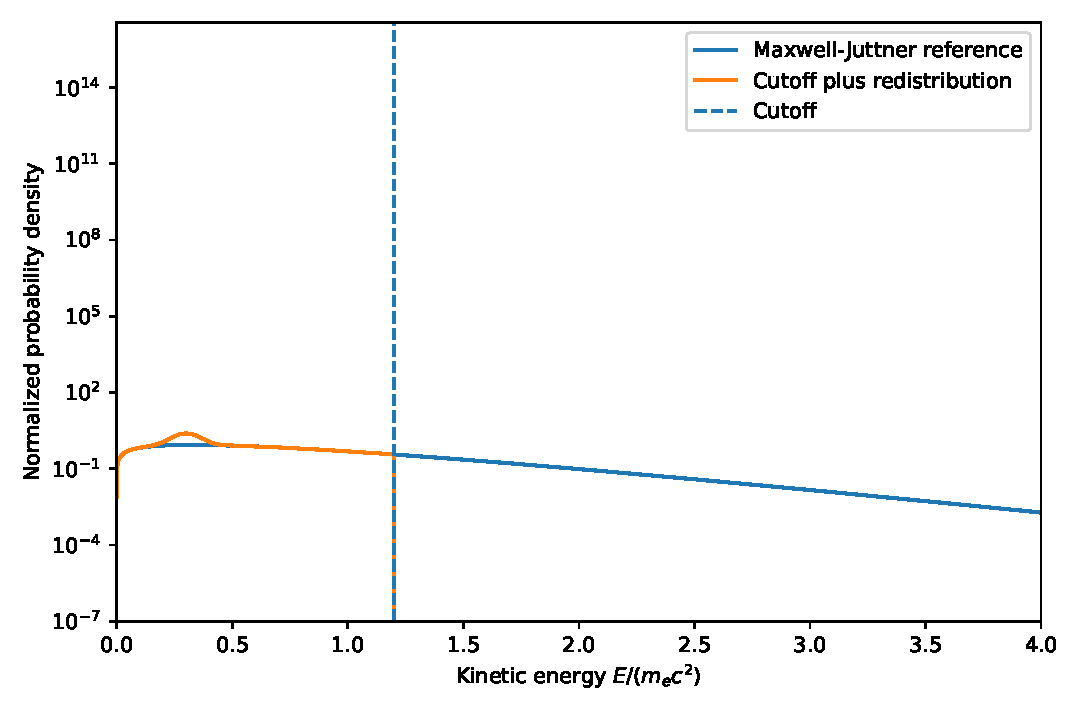
\includegraphics[width=0.78\textwidth]{distribution_cutoff.pdf}
\caption{Normalized Maxwell--J\"uttner reference distribution and a number-conserving cutoff-plus-redistribution example. The deposited low-energy feature is a numerical representation of particles transferred from the superthermal tail.}
\label{fig:distribution-cutoff}
\end{figure}

The model preserves particle number to numerical precision. It does not preserve electron energy because the control mechanism is presumed to transfer the difference to another reservoir. A realistic simulation would track that reservoir explicitly.

\section{Tail fraction and radiation-weighted moments}

The tail number fraction is
\begin{equation}
F_N(E_c)=\int_{E_c}^{\infty}p(E)\,\dd E.
\end{equation}
For the selected relativistic temperature, a cutoff at only a few $k_BT_e$ can contain a non-negligible particle fraction because the relativistic density-of-states factor shifts the energy distribution. This illustrates why a proposed cutoff must be defined in physical energy and not interpreted from nonrelativistic intuition alone.

\begin{table}[H]
\centering
\caption{Illustrative number fractions and radiation-weighted moment ratios at $\theta=0.40$. $M_q$ is defined by Equation~\eqref{eq:moment}. Values are generated by the included script and are not full bremsstrahlung power ratios.}
\label{tab:moment-results}
\begin{tabular}{ccccc}
\toprule
$E_c/k_BT_e$ & Tail number fraction & $M_1/M_{1,0}$ & $M_2/M_{2,0}$ & $M_3/M_{3,0}$ \\
\midrule
1.5 & 0.546 & 0.322 & 0.0816 & 0.0181 \\
2.0 & 0.409 & 0.440 & 0.154 & 0.0468 \\
3.0 & 0.215 & 0.614 & 0.324 & 0.152 \\
4.0 & 0.107 & 0.758 & 0.515 & 0.313 \\
5.0 & 0.051 & 0.861 & 0.682 & 0.490 \\
\bottomrule
\end{tabular}
\end{table}

The table demonstrates the central mathematical effect. For a $5k_BT_e$ cutoff, only about five percent of particles are moved in this illustrative distribution, yet the cubic energy moment falls by roughly one half. The exact bremsstrahlung kernel is not $E^3$, but higher-energy electrons contribute disproportionately, so moment reduction is a useful screening metric.

\begin{figure}[H]
\centering
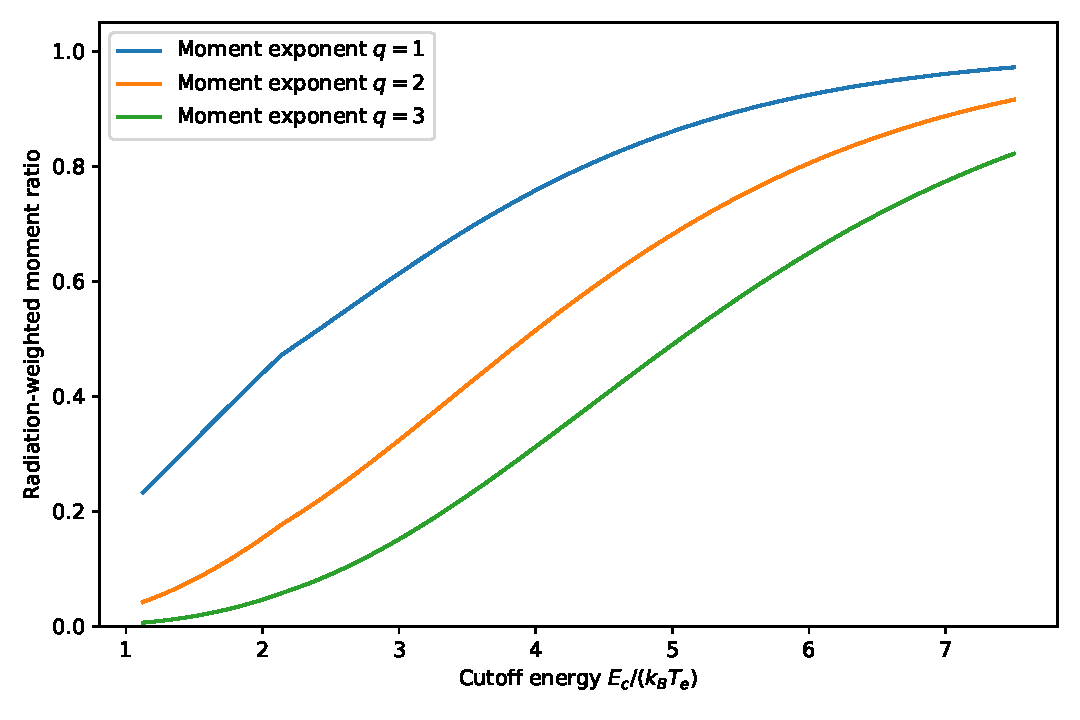
\includegraphics[width=0.78\textwidth]{moment_reduction.pdf}
\caption{Radiation-weighted moment ratio versus cutoff energy for three surrogate energy exponents. More strongly energy-weighted processes benefit more from removal or redistribution of the tail.}
\label{fig:moment-reduction}
\end{figure}

\section{Interpretation for electron--ion and electron--electron emission}

Electron--ion bremsstrahlung can be represented as a one-electron average over an energy-dependent cross-section kernel. Electron--electron emission is a two-electron average and becomes more important as relativistic particles become common. The illustrative moment result suggests two qualitative expectations:
\begin{enumerate}
\item both channels decrease when high-energy electrons are moved to lower energy; and
\item electron--electron emission may respond especially strongly because encounters involving two energetic electrons are depleted.
\end{enumerate}
These expectations are consistent with relativistic calculations showing suppression under tail redistribution \cite{munirov2023}. Their magnitude must be computed using the actual cross sections and angular distribution.

\section{A surrogate spectral calculation}

To demonstrate spectral weighting, the baseline source is represented by
\begin{equation}
S_0(E_\gamma)\propto E_\gamma e^{-E_\gamma/k_BT_e},
\end{equation}
which has a bremsstrahlung-like continuum shape but is not an exact emissivity. A smooth suppression factor is applied preferentially above a cutoff-dependent photon energy. Three response functionals are then compared:
\begin{enumerate}
\item integrated energy fluence;
\item a shallow-tissue weighting that emphasizes lower photon energy; and
\item a penetrating-dose weighting that emphasizes higher photon energy.
\end{enumerate}
The weightings are intentionally dimensionless surrogates. In a real calculation they are replaced by Monte Carlo transport and mass energy-absorption coefficients.

\begin{figure}[H]
\centering
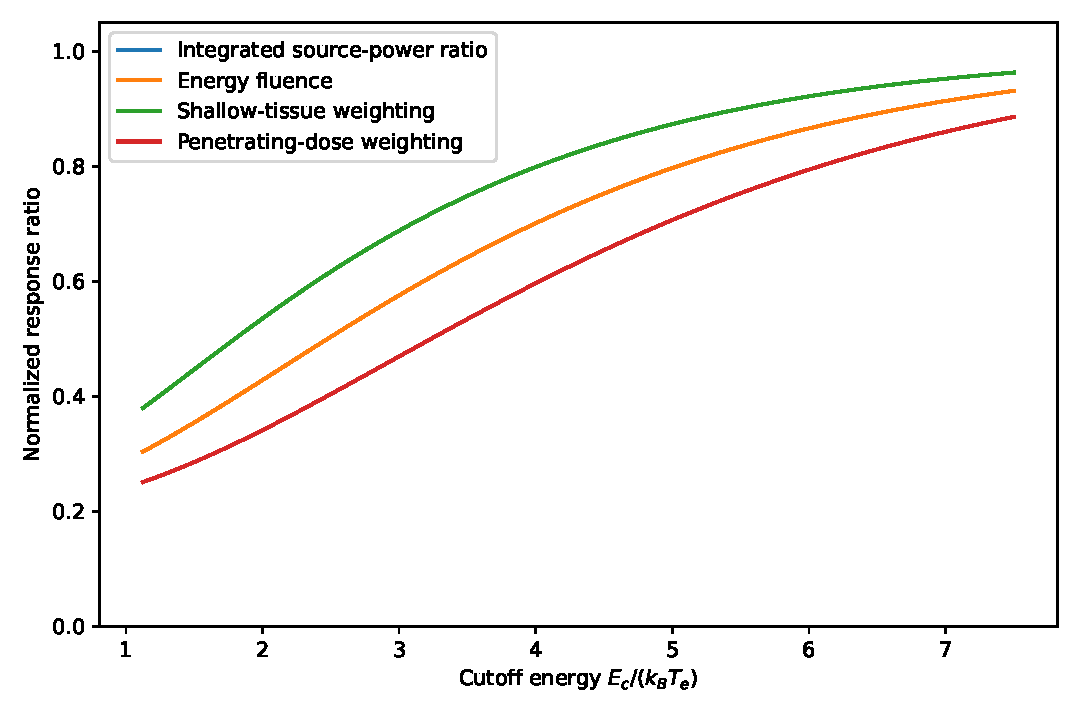
\includegraphics[width=0.78\textwidth]{dose_vs_power.pdf}
\caption{Illustrative comparison of integrated source reduction and spectrally weighted response. Different receptors need not experience the same reduction even when exposed to the same modified source.}
\label{fig:dose-vs-power}
\end{figure}

\Cref{fig:dose-vs-power} shows that the response ratio depends on the spectral weighting. In this particular constructed example, high-energy suppression produces a larger decrease in the penetrating-dose functional than in the shallow-energy-weighted functional. A different spectral suppression could reverse the ordering. The robust conclusion is not the specific curve; it is that the downstream receptor changes the benefit metric.

\section{First-order biological response}

If magnetic control changes dose but not radiation quality, oxygenation, or dose-rate response, the linear-quadratic model predicts
\begin{equation}
\frac{S_c}{S_0}
=\exp\left[-\alpha(D_c-D_0)-\beta(D_c^2-D_0^2)\right].
\label{eq:survival-ratio}
\end{equation}
Because $D_c<D_0$, the controlled-source surviving fraction is higher for normal tissue or unintended exposure. The response is nonlinear: a fifty-percent dose reduction can yield much more than a fifty-percent change in surviving fraction when the baseline dose lies on the steep part of the survival curve.

For occupational low-dose exposure, clonogenic survival is not the relevant risk endpoint. A protection-model estimate instead scales collective or individual risk approximately with effective dose under the adopted low-dose model. Thus, the same physical source reduction has application-specific biological interpretation.

\section{Illustrative foci kinetics}

For an acute exposure with initial DSB proxy $N_0=Y_DD$, single-exponential repair gives
\begin{equation}
N(t)=Y_DD e^{-k_rt}+N_{\mathrm{res}},
\label{eq:foci}
\end{equation}
where $N_{\mathrm{res}}$ represents persistent lesions or background. If source suppression only reduces dose, all time points scale approximately with $D$ after background subtraction. If the initial foci ratio equals the dose ratio but the late foci ratio differs, the spectrum or dose-rate change may have altered lesion complexity or repair. This is why time-resolved foci are more informative than a single time point.

\section{Energy-balance test}

Suppose the plasma-volume bremsstrahlung power decreases by $\Delta P_{\mathrm{plasma}}<0$, while redirected electrons produce collector radiation $\Delta P_{\mathrm{collector}}>0$. Net source suppression requires
\begin{equation}
\Delta P_{\mathrm{external}}
=\Delta P_{\mathrm{plasma}}
+\Delta P_{\mathrm{collector}}
+\Delta P_{\mathrm{secondary}}<0.
\end{equation}
For biological dose at receptor $r$, the stronger condition is
\begin{equation}
\int K_r(E,\Omega,\mathbf{x})\Delta j_{\mathrm{external}}\,
\dd E\dd\Omega\dd^3x<0.
\end{equation}
A collector can emit less total power than the original plasma while creating a more directional source near a penetration. The dose-kernel condition therefore supersedes an integrated-power condition.

\section{Sensitivity expectations}

The model predicts strong sensitivity to:
\begin{itemize}
\item cutoff energy and transition sharpness;
\item location of redistributed particles;
\item electron temperature and anisotropy;
\item impurity $Z_{\mathrm{eff}}$;
\item the fraction of lost electrons intercepted by high-$Z$ material;
\item source directionality and receptor geometry; and
\item low-energy filtration and high-energy streaming paths.
\end{itemize}
The model predicts weaker sensitivity to parameters that affect only low-energy bulk electrons when the biological receptor is dominated by penetrating hard photons. Global sensitivity analysis should test, rather than assume, this ordering.

\section{Falsifying outcomes}

The proposed mechanism would be weakened or rejected if:
\begin{enumerate}
\item the measured tail is unchanged while the detector signal falls, suggesting geometry or calibration effects;
\item electron--electron or collector emission compensates for the electron--ion reduction;
\item synchrotron power increases by more than bremsstrahlung decreases;
\item the residual spectrum hardens enough that receptor dose does not decrease;
\item equal-dose biological response differs in a way inconsistent with measured spectrum and pulse structure; or
\item perturbation-induced confinement loss reduces fusion output more than the radiative saving.
\end{enumerate}
A useful thesis must make these failure conditions explicit.

\section{Summary}

The illustrative calculations establish three robust trends: tail redistribution can strongly reduce energy-weighted moments; the benefit is larger for more strongly energy-weighted channels; and biological dose reduction is a receptor-weighted spectral quantity rather than a synonym for total-power reduction. These results justify the full cross-section, transport, and validation program.

\chapter{Applications to Fusion, Plasma Radiation Sources, and Biological Exposure}
\label{ch:applications}

\section{Proton--boron-11 fusion}

The \pB \ reaction
\begin{equation}
p+{}^{11}\mathrm{B}\rightarrow 3\alpha+8.68\ \mathrm{MeV}
\end{equation}
is attractive because the primary products are charged and the fuel constituents are comparatively abundant. The reaction is often described as aneutronic, but a complete reactor assessment must include secondary reactions, impurities, activation, and high-energy photons. The central energy-balance obstacle is that useful reactivity requires temperatures at which electron radiation is severe \cite{rider1995,nevins2000,sikora2016,ochs2022}.

Distribution engineering addresses the problem at its physical origin. A reactor may seek hot or fast ions near the reaction-energy range while maintaining cooler electrons, redirecting alpha energy into ions, and suppressing the superthermal electron tail. Magnetic perturbations could contribute by selectively deconfining radiatively costly electrons or by coupling them to wave and electrostatic structures that transfer energy elsewhere. However, electrons also provide ambipolar confinement, current, quasi-neutrality, and collisional coupling. Overaggressive removal can deepen potentials, drive replacement heating, destabilize the plasma, or increase ion losses.

The radiobiological extension matters for plant design. Even if \pB \ reduces neutron shielding requirements relative to deuterium--tritium, bremsstrahlung can dominate prompt dose outside the plasma. Source-term control may reduce shield thickness, maintenance dose, diagnostic saturation, and occupational exposure. These benefits must be quantified spectrally because low-energy X rays are easily shielded but can produce high local dose near thin windows, while hard photons dominate deep penetration and streaming.

\section{Mirror and open-field-line systems}

Mirror machines provide a natural environment for energy-selective escape. The loss cone, mirror ratio, ambipolar potential, and relativistic confinement scaling determine which electrons leave \cite{pastukhov1974,ochs2023mirror}. A controlled perturbation can enlarge the loss region for a selected phase-space population. The engineering advantage is that open ends provide intentional collection geometry; the disadvantage is that end losses can be large and produce intense localized radiation when electrons strike hardware.

A mirror implementation should include an expanding magnetic nozzle, electrostatic energy recovery where feasible, and low-$Z$ electron collectors. Diagnostics placed along the end loss channel can directly measure the removed distribution, providing a strong validation of the cutoff mechanism. Biological dose should be evaluated both radially and along the axis, where streaming is most likely.

\section{Tokamaks and stellarators}

Resonant magnetic perturbations are established tools for modifying edge topology in toroidal confinement \cite{evans2004,fitzpatrick1993,wesson2011}. Applying them to bremsstrahlung suppression is more difficult because the energetic population may be core localized, while broad stochasticity degrades energy confinement. A feasible concept would target an energetic-electron subpopulation with mode structure, frequency, and radial localization that minimize bulk transport.

Runaway-electron physics provides a cautionary analogy. Synchrotron and bremsstrahlung reaction can limit runaway energy, while magnetic perturbations can deconfine runaways, but localized wall impacts create severe material loads. The same trade-off appears here: removal of radiating electrons must not convert a diffuse photon source into an unacceptable localized electron beam. Bremsstrahlung reaction also reshapes the distribution and should be retained in any runaway-like regime \cite{embreus2016}.

\section{Laser-produced plasmas}

High-intensity lasers generate nonthermal electrons through resonance absorption, $\mathbf{J}\times\mathbf{B}$ heating, wakefield processes, and sheath acceleration. These electrons create bremsstrahlung when traversing dense plasma or solid targets. Laser-driven \pB \  experiments have demonstrated energetic alpha production, but conversion efficiency, electron heating, target geometry, and radiation losses remain central challenges \cite{labaune2013,picciotto2014,giuffrida2020}.

External magnetic fields can guide electron transport, modify filamentation, and alter refluxing in the target. The proposed framework can evaluate whether a magnetic field reduces source bremsstrahlung in the interaction region or merely redirects electrons to a new converter location. Because laser sources are strongly pulsed and directional, time-resolved dosimetry and angular spectra are indispensable. Extremely high instantaneous dose rate does not automatically imply a beneficial FLASH response in nearby tissue; the field may be spatially nonuniform, mixed with particles, and delivered at a total dose outside therapeutic conditions.

\section{Dense plasma focus and Z-pinch devices}

Dense plasma focus and Z-pinch systems produce intense pulsed X rays, electron beams, ions, and in some operating modes neutrons \cite{haines2011,lee2014}. Their compactness has motivated study as radiography and ultra-high-dose-rate radiation sources \cite{sumini2019,isolan2022}. Magnetic perturbations are inherent in the pinch dynamics, and instability controls may alter both plasma confinement and radiation output.

For radiobiology, these devices are valuable test beds because they naturally couple plasma physics to pulsed exposure. They also illustrate the need for mixed-field characterization. A measured biological effect cannot be attributed to X rays without excluding electrons, ions, neutrons, ultraviolet radiation, electromagnetic pulse artifacts, sample heating, and mechanical shock. The full methodology in \Cref{ch:methodology} is especially relevant.

\section{Accelerator and beam-plasma systems}

Relativistic electron beams interacting with plasma or high-$Z$ targets generate tunable bremsstrahlung. Wakefield accelerators and beam-driven plasma sources can produce compact ultrashort X-ray pulses. Magnetic optics shape the electron beam before conversion; plasma-based magnetic structures may also influence energy spread and divergence. Distribution-function engineering can reduce unwanted halo electrons or select the energy range that contributes to a desired photon spectrum.

In an intentional radiation source, ``suppression'' is not always the objective. The same framework can optimize spectral quality: reduce biologically inefficient or shielding-intensive components while retaining photons useful for imaging, therapy, or materials testing. The biological weighting in Equation~\eqref{eq:bio-objective} can be replaced by image-quality or detector-response weighting when appropriate.

\section{Medical and preclinical radiation research}

Plasma-generated photon sources may serve radiobiology or radiotherapy research if they can deliver calibrated, reproducible fields. Their possible advantages include compact geometry, short pulses, and unconventional spectra. Their barriers include source instability, dose-rate metrology, field uniformity, mixed radiation, and regulatory complexity.

A source designed for preclinical use should be benchmarked against conventional kilovoltage or megavoltage X rays using traceable dosimetry and biological endpoints. The linear-quadratic model, oxygen effect, Relative Biological Effectiveness (RBE), and tissue constraints remain relevant, but nonstandard pulse structure may require additional modeling. A direct transition to patient treatment would be premature without extensive dosimetric, toxicological, engineering, and clinical validation.

\section{Space and aerospace applications}

High-energy plasma and accelerator systems used in space propulsion, radiation testing, or compact power concepts can create ionizing radiation. Space radiation biology is usually dominated by trapped particles, solar particles, and galactic cosmic rays, but local device-generated photons and particles can add to crew or electronics dose. The source-to-biology framework supports onboard optimization: magnetic topology can be evaluated simultaneously for device performance, vehicle shielding, crew location, and mission duty cycle.

For crew protection, equivalent and effective dose are more relevant than in vitro survival. Mixed fields require radiation-quality weighting and organ geometry. The framework also applies to ground testing, where pulsed plasma devices may expose operators through direct lines of sight or shield penetrations.

\section{Occupational radiation protection}

A facility safety analysis begins with source identification and proceeds through engineered controls, administrative controls, and personal monitoring. The protection principles are justification, optimization, and limitation, implemented through time, distance, shielding, interlocks, access control, surveys, and ALARA planning \cite{icrp103,iaeaGSR3}. Magnetic source suppression is an engineered control, but it does not eliminate the need for passive shielding or monitoring because the control can fail or operate outside its validated range.

Operational dose should be evaluated for normal operation, commissioning, maintenance, credible faults, and post-shutdown activation. Source suppression may reduce prompt dose but not residual activation. Conversely, reduced photon heating can lower activation indirectly by permitting different materials or operating conditions. These couplings are facility specific.

\section{Environmental and public exposure}

Public exposure from a well-designed plasma facility should be dominated by controlled emissions and shielding leakage rather than direct access to the source. The relevant analysis uses annual operation, occupancy, skyshine where applicable, effluents, activation, and accident scenarios. A reduction in bremsstrahlung source term can reduce off-site dose, but the public-dose consequence must be calculated with site geometry and regulatory models rather than inferred from laboratory detector ratios.

Environmental radiobiology also considers non-human biota, radionuclide transport, and ecosystem effects \cite{baatout2023,unscear2020}. For a nominally aneutronic system, radionuclide inventories may be smaller than in neutron-rich fusion, but secondary sources and activated components still require characterization.

\section{Electronics and instrumentation}

Radiation damage is not only biological. X rays and secondary electrons cause ionization in detectors, cables, insulators, semiconductors, and control electronics. Total ionizing dose, single-event effects from secondary particles, displacement damage, and detector saturation can limit operation. A spectral source reduction may extend component life and improve diagnostic dynamic range even when worker dose is already acceptable.

The same transport matrix can produce component dose. Biological weighting is replaced by material energy deposition, displacement-damage functions, or device response. This dual use strengthens the case for preserving spectral information throughout the model.

\section{Design case study: source suppression versus additional shielding}

Consider two options for reducing dose at a maintenance location:
\begin{description}
\item[Option A:] magnetic control reduces the hard-photon source by a factor $R_S(E)$ but adds coil power, complexity, and electron collector load;
\item[Option B:] additional passive shielding changes the transport operator but leaves plasma performance unchanged.
\end{description}
The decision compares lifecycle cost, reliability, dose, mass, access, heat, activation, and maintainability. Source suppression may be superior for streaming through many penetrations because it acts before geometric branching. Shielding may be superior if the perturbation degrades fusion performance or creates new local sources. A hybrid design often dominates: moderate source reduction followed by optimized graded shielding.

\section{Summary}

The unified framework applies across advanced fusion, mirror systems, toroidal devices, laser plasmas, dense plasma focus sources, accelerator systems, medicine, space, and occupational protection. The specific objective changes, but the logic remains constant: control the particle distribution, calculate the complete external source, transport it to a defined receptor, and use an endpoint-appropriate response model.

\chapter{Discussion}
\label{ch:discussion}

\section{Interpretation of the central thesis}

The central claim of this work is not that magnetic fields directly neutralize ionizing radiation. Magnetic fields do not attenuate photons in the manner of lead, concrete, or water. The claim is that a controlled magnetic perturbation can alter the charged-particle distribution that creates the photons. If the superthermal electron population is depleted, redirected, or decelerated before radiative encounters occur, the photon source term can decrease. Radiation biology then provides the consequence model needed to determine whether that physical reduction improves safety or changes biological response.

This distinction separates source-term engineering from shielding. Shielding acts after emission and is constrained by mass, space, activation, heat, penetrations, and secondary radiation. Source-term engineering acts before or during emission and is constrained by plasma stability, confinement, current balance, and energy flow. The strategies are complementary. A robust design uses source control to reduce the burden on shielding while retaining shielding for defense in depth.

\section{Why the high-energy tail is a leverage point}

The high-energy tail is attractive because it can carry a disproportionate share of relativistic radiative power. The illustrative results in \Cref{ch:model-results} show that high-order energy moments can fall much more than particle number when tail electrons are redistributed. Full bremsstrahlung kernels are more complex than polynomial moments, but published relativistic calculations support the qualitative conclusion that superthermal redistribution can suppress radiation \cite{munirov2023}.

The leverage is not free. Tail electrons may contribute to current drive, ambipolar potentials, wave damping, alpha-channeling pathways, or diagnostic signals. Their removal can alter the entire plasma. The most favorable case is one in which the radiatively expensive population contributes little to the desired fusion or confinement function. The least favorable case is one in which the same electrons are essential for stability or power transfer.

\section{Magnetic perturbations as a control mechanism}

Magnetic perturbations offer several routes to selectivity: resonance, finite-orbit-width effects, stochastic edge layers, loss-cone diffusion, and altered access to electrostatic potentials. The broad class is physically plausible because perturbations are already used to alter transport in magnetized plasmas \cite{rechester1978,fitzpatrick1993,evans2004}. The unanswered question is whether sufficiently strong selectivity can be achieved without unacceptable bulk-confinement loss.

A static perturbation may provide spatial selectivity but limited direct energy exchange. A rotating or wave-like perturbation can provide phase-space selectivity and induced electric fields, yet also risks acceleration. Mirror geometries are especially promising because open ends and loss cones naturally separate confined and escaping populations. Toroidal devices offer mature perturbation technology but may have less tolerance for core stochasticity.

The phrase ``utilizing magnetic perturbations'' should therefore be interpreted as a family of kinetic control schemes, not a single coil configuration. The thesis contributes the criteria by which candidate schemes can be compared.

\section{The importance of energy closure}

The most serious conceptual error would be to treat removed tail energy as if it vanished. If electrons escape, they carry kinetic energy. If they are decelerated, fields or circuits receive energy. If they thermalize, bulk electrons or ions are heated. If they strike a collector, they generate heat and radiation. A successful scheme closes both particle and energy balances.

This closure is especially important for biological claims. Plasma-volume bremsstrahlung may fall while collector bremsstrahlung rises in a direction that increases local dose. The total source must include all components in Equation~\eqref{eq:total-source}. The dose-kernel formulation then weights their location and direction.

\section{Why radiated power and biological effect diverge}

Biological effect is not a direct meter of source power. Between source and cell lie geometry, shielding, spectral attenuation, secondary-electron transport, dose rate, and biological context. A low-energy photon removed from the source may have contributed strongly to entrance dose but little to a deeply shielded receptor. A high-energy photon may contribute relatively little to local source power yet dominate dose beyond thick shielding. Therefore, source optimization should use the receptor-specific kernel of Equation~\eqref{eq:dose-kernel}.

The divergence does not mean plasma engineers must become clinical radiobiologists for every calculation. A tiered approach is sufficient:
\begin{enumerate}
\item use total power for plasma energy balance;
\item use spectral dose for shielding and receptor calculations;
\item use equivalent/effective dose for protection planning; and
\item use endpoint-specific radiobiology for experiments or therapy.
\end{enumerate}
Confusion arises when a quantity from one tier is used as a substitute for another.

\section{Radiation quality of plasma-generated photons}

For most bremsstrahlung photon fields, low-LET models are appropriate. Yet the broad spectrum can range from soft X rays to multi-MeV photons, producing secondary electrons with different energies and ranges. Equal absorbed dose from two photon spectra may not be exactly biologically equivalent, especially when comparing kilo-voltage and mega-voltage beams or very small targets. This is why the proposed study includes a dose-matched biological comparison.

A measured difference at equal dose should not be attributed immediately to a novel plasma effect. Possible explanations include dosimeter energy dependence, dose gradients in the culture vessel, pulse-response error, oxygen changes, electromagnetic interference, sample heating, and mixed-particle contamination. Only after these are excluded should a radiation-quality or dose-rate mechanism be inferred.

\section{Implications for advanced-fuel fusion}

For \pB \ fusion, the framework re-frames bremsstrahlung as both an internal efficiency loss and an external radiological source. A distribution-control strategy has dual value if it improves the fusion power balance and reduces shielding burden. It has limited value if it reduces measured X rays but sacrifices more fusion power through particle loss. The correct figure of merit combines fusion gain, radiative loss, wall load, and receptor dose.

Recent work on alpha channeling and non-thermal proton schemes shows that controlling energy flow among species can substantially change the feasibility margin \cite{ochs2022}. Tail suppression is conceptually aligned with this program: keep energy in fusion-productive ions and out of radiatively costly electrons. Magnetic perturbations could support that goal, but their interaction with alpha confinement and wave dynamics requires coupled modeling.

The ``aneutronic'' advantage should be expressed cautiously. Primary neutron production is reduced, not every radiological hazard. Bremsstrahlung, secondary nuclear reactions, activation, and lost charged particles remain. A credible safety case quantifies each.

\section{Comparison with conventional radiation protection}

Conventional radiation protection relies on source control wherever feasible, followed by engineered barriers and administrative measures. Magnetic suppression fits naturally at the top of this hierarchy as an engineered source-reduction measure. Its novelty lies in using kinetic plasma control rather than mechanical containment or process substitution.

However, a source-control system that depends on active coils, power supplies, feedback, and plasma state has failure modes. Passive shielding remains necessary for credible loss of control. Radiation monitors should verify that the source remains within the validated envelope. Interlocks can use hard-X-ray signals, coil status, and plasma diagnostics to terminate operation if suppression fails.

\section{Limitations of the present thesis}

\subsection{No new experimental dataset}

The thesis provides a theoretical and methodological framework, not unreported experimental proof. The illustrative results are normalized surrogate calculations. A final experimental thesis must replace or supplement them with measured distributions, spectra, dose, and biological endpoints.

\subsection{Reduced radiation kernels}

The illustrative moment and spectral models do not substitute for exact electron--ion and electron--electron differential cross sections. Full calculations must include screening, Coulomb corrections, anisotropy, composition, and relativistic kinematics.

\subsection{Simplified magnetic loss operator}

The energy-dependent loss rate is phenomenological until calibrated by orbit following or kinetic simulation in a specific geometry. Plasma response can screen or amplify the applied perturbation.

\subsection{Biological model reduction}

The linear-quadratic model and simple repair equations are useful but incomplete. They do not represent the full DNA damage response, immune system, vascular injury, organ architecture, or long-term carcinogenesis. Protection quantities and cellular endpoints must remain conceptually separate.

\subsection{Facility specificity}

Shielding and dose conclusions depend strongly on geometry, material, duty cycle, and receptor location. The framework is transferable; numerical dose values are not.

\section{Alternative explanations and confounders}

An apparent reduction in X-ray signal after applying a perturbation could be caused by:
\begin{itemize}
\item lower plasma density or stored energy;
\item changed detector line of sight;
\item angular redistribution rather than reduced total emission;
\item electromagnetic interference with the detector;
\item detector saturation in one condition;
\item increased self-absorption;
\item altered impurity concentration;
\item timing jitter relative to the acquisition gate; or
\item source displacement.
\end{itemize}
The experimental design includes diagnostics and normalizations to distinguish these alternatives.

A lower biological response could be caused by lower dose, but also by altered sample temperature, oxygenation, handling time, electromagnetic fields, or selection bias. Sham perturbation controls and a conventional reference beam are therefore necessary.

\section{What would constitute strong evidence}

Strong evidence would consist of a coherent chain:
\begin{enumerate}
\item orbit and kinetic models predict an energy-selective loss region;
\item independent diagnostics observe the corresponding tail depletion;
\item absolute, angle-resolved spectra show the predicted channel-specific reduction;
\item collector and wall sources are included and the external source decreases;
\item Monte Carlo transport predicts a receptor-dose reduction;
\item calibrated phantom measurements confirm it; and
\item biological endpoints follow the dose prediction without configuration-specific refitting.
\end{enumerate}
Such a result would justify the claim that magnetic perturbations reduce biologically relevant radiation emissions, not merely one diagnostic signal.

\section{Unexpected but scientifically useful outcomes}

Several negative outcomes would still advance the field. If magnetic perturbations reduce bremsstrahlung but increase synchrotron, the result identifies a coupled optimization constraint. If the plasma source decreases but collector radiation dominates, it motivates energy recovery or low-$Z$ collection. If dose decreases less than power because the residual spectrum hardens, it demonstrates the need for biological weighting. If equal-dose biological response is unchanged, that supports the use of conventional low-LET models. If it differs, the result motivates detailed microdosimetry and pulse-chemistry studies.

\section{Future theoretical work}

Priority theoretical developments are:
\begin{enumerate}
\item full relativistic two-dimensional Fokker--Planck modeling with self-consistent radiation reaction;
\item orbit-derived loss operators in measured three-dimensional fields;
\item coupled plasma-wall electron transport and target bremsstrahlung;
\item adjoint source-to-dose kernels for control optimization;
\item multi-objective optimization including fusion gain and radiological consequence; and
\item uncertainty-aware reduced-order models suitable for real-time feedback.
\end{enumerate}

\section{Future experimental work}

The first experiment should be modest and decisive rather than attempting a reactor-scale demonstration. A mirror or linear magnetized plasma with a measurable nonthermal electron tail, controllable perturbation coils, hard-X-ray diagnostics, and a dedicated low-$Z$ collector would provide a clean test. The biological validation can be performed downstream using a phantom and cell cultures only after the physical source and dose are stable.

A second phase could use a dense plasma focus or laser-plasma source to examine pulse structure and mixed fields. A third phase could integrate the method into an advanced-fuel fusion experiment.

\section{Summary}

The thesis establishes a rigorous interpretation of magnetic radiation suppression. The physics is plausible and potentially valuable, but the benefit must survive energy closure, complete source accounting, spectral transport, and biological validation. The strongest contribution is the unified criterion: a successful perturbation reduces the relevant external source and its receptor-weighted consequence while preserving the intended plasma function.

\chapter{Conclusions and Future Work}
\label{ch:conclusions}

\section{Conclusions}

This thesis developed a unified framework for evaluating the biological implications of suppressing radiation emissions from relativistic plasmas by means of magnetic perturbations. The analysis began with the electron distribution function, retained electron--ion and electron--electron bremsstrahlung, incorporated competing synchrotron emission, transported the resulting photon spectrum through matter, converted spectral fluence to absorbed dose, and connected dose to molecular and cellular response.

The principal conclusions are as follows.

First, relativistic bremsstrahlung is highly sensitive to the superthermal electron population. A small population fraction can contribute a much larger fraction of an energy-weighted radiation metric. Number-conserving redistribution to lower energy therefore has the potential to reduce radiative losses, consistent with published relativistic analyses \cite{munirov2023}.

Second, magnetic perturbations can create an effective cutoff only indirectly. They alter topology, resonance, pitch-angle diffusion, access to loss cones, electrostatic potentials, or boundaries. The magnetic field itself does no work; energy reduction requires induced electric fields, collisional relaxation, escape, or transfer to another reservoir. Any credible model must close particle and energy balances.

Third, plasma-volume suppression is insufficient as a system metric. Lost electrons can produce bremsstrahlung at collectors or walls, magnetic control can increase synchrotron emission, and the residual photon spectrum can become more penetrating. The correct source term includes plasma, collector, activation, neutron, and other secondary components.

Fourth, biological benefit is spectrally and geometrically weighted. A reduction in total photon power does not necessarily produce the same reduction in absorbed dose. The dose ratio is a weighted integral of the spectral suppression after transport. The receptor, shielding, and tissue composition determine the weighting.

Fifth, radiation biology provides a validation ladder rather than a single conversion coefficient. Physical dosimetry should be followed by early DNA-damage markers, cytogenetic endpoints, and clonogenic survival. Source-normalized comparisons demonstrate dose reduction; dose-matched comparisons test whether spectral or temporal changes alter biological effectiveness.

Sixth, the method is most persuasive when validated as a chain. Independent electron diagnostics must confirm tail control; absolute spectra must confirm source reduction; energy accounting must exclude compensating sources; transport and phantom dosimetry must confirm dose reduction; and biological endpoints must agree without configuration-specific refitting.

Finally, the framework is broadly applicable. It can be used for \pB fusion, mirror systems, toroidal confinement, laser-produced plasmas, dense plasma focus devices, accelerator sources, radiation research, space systems, electronics protection, and occupational safety. The application-specific endpoint changes, but the source-to-consequence logic remains the same.

\section{Recommended next phase}

The recommended next phase is a staged physical validation rather than immediate biological experimentation.

\begin{enumerate}
\item Select a plasma device with a stable measurable nonthermal electron tail and controllable magnetic perturbations.
\item Map the vacuum and plasma-response fields and perform relativistic orbit following.
\item Build a reduced Fokker--Planck model with an orbit-calibrated loss operator.
\item Measure the unperturbed and perturbed electron distributions using at least two independent diagnostics.
\item Measure absolute spectral-angular photon output and collector radiation.
\item Close the energy balance and verify that total external radiation decreases.
\item Construct a validated transport model and tissue-equivalent phantom.
\item Only then perform cell exposures with a conventional reference beam and both source-normalized and dose-matched comparisons.
\end{enumerate}

This sequence minimizes the risk that biological variability obscures an unresolved plasma or dosimetry problem.

\section{Specific future research questions}

Future work should answer:
\begin{enumerate}
\item What perturbation spectrum maximizes superthermal-electron loss selectivity while preserving bulk confinement?
\item Can escaping electron energy be recovered electrostatically rather than deposited in a collector?
\item How strongly does electron--electron bremsstrahlung respond relative to electron--ion emission in the experimentally achieved distribution?
\item Does the residual spectrum harden, soften, or develop angular lobes?
\item Under what conditions does synchrotron power offset bremsstrahlung suppression?
\item Can adjoint dose kernels be integrated into real-time magnetic feedback?
\item Do equal absorbed doses from baseline and controlled plasma spectra produce indistinguishable low-LET biological response?
\item How does the optimum change when fusion gain, shield mass, component dose, and worker dose are optimized simultaneously?
\end{enumerate}

\section{Final perspective}

Radiation control in a relativistic plasma can be approached at three levels: after emission with shielding, during transport with geometry and collimation, or before emission by controlling the particles that radiate. Magnetic perturbations offer a route to the third level. Their value will not be established by a reduction in one X-ray channel alone, but by a complete demonstration that the controlled plasma performs its intended function while the external, transported, and biologically relevant radiation field decreases.

The integration of plasma physics and radiation biology is therefore not an artificial merger of disciplines. It is the natural completion of the causal chain from charged-particle dynamics to human and material consequence.


\begin{appendices}
\chapter{Selected Derivations}
\label{app:derivations}

\section{Normalization of the Maxwell--J\"uttner distribution}

For an isotropic distribution,
\begin{equation}
 n_e=4\pi\int_0^\infty p^2 f(p)\,\dd p.
\end{equation}
Let $u=p/(m_ec)$ and $\gamma=\sqrt{1+u^2}$. The integral identity
\begin{equation}
\int_0^\infty u^2e^{-\gamma/\theta}\,\dd u
=\theta K_2(1/\theta)
\end{equation}
leads to Equation~\eqref{eq:mj}. The energy density is
\begin{equation}
U_e=4\pi\int_0^\infty p^2(\gamma-1)m_ec^2f(p)\,\dd p.
\end{equation}

\section{Number-conserving redistribution}

Starting from normalized $f_0(E)$, define
\begin{equation}
N_>=\int_{E_c}^{\infty}f_0(E)\dd E.
\end{equation}
For a normalized redistribution kernel $g_r$, the new distribution is
\begin{equation}
f_c(E)=f_0(E)H(E_c-E)+N_>g_r(E).
\end{equation}
Then
\begin{align}
\int_0^\infty f_c(E)\dd E
&=\int_0^{E_c}f_0(E)\dd E+N_>\\
&=1-N_>+N_>=1.
\end{align}
The energy change is
\begin{equation}
\Delta\langle E\rangle
=N_>\langle E\rangle_r-\int_{E_c}^{\infty}Ef_0(E)\dd E,
\end{equation}
which is negative when the redistribution mean lies below the original tail mean.

\section{Dose ratio as a weighted spectral average}

Let the controlled source be $S_c(E)=R_S(E)S_0(E)$. For a fixed linear transport and dose weighting $W(E)$,
\begin{equation}
D_0=\int W(E)S_0(E)\dd E,
\qquad
D_c=\int W(E)R_S(E)S_0(E)\dd E.
\end{equation}
Therefore
\begin{equation}
\frac{D_c}{D_0}
=\int R_S(E)\pi_D(E)\dd E,
\end{equation}
where
\begin{equation}
\pi_D(E)=\frac{W(E)S_0(E)}{\int W(E')S_0(E')\dd E'}
\end{equation}
is a normalized nonnegative weighting density. Thus $D_c/D_0$ lies between the minimum and maximum of $R_S$ over the contributing energy range. It equals the total-power ratio only for special weightings or spectrally uniform suppression.

\section{Linear-quadratic survival under dose reduction}

For baseline and controlled doses $D_0$ and $D_c$,
\begin{equation}
\ln\left(\frac{S_c}{S_0}\right)
=-\alpha D_c-\beta D_c^2+\alpha D_0+\beta D_0^2.
\end{equation}
Factorization gives
\begin{equation}
\ln\left(\frac{S_c}{S_0}\right)
=(D_0-D_c)\left[\alpha+\beta(D_0+D_c)\right].
\end{equation}
For nonnegative $\alpha$, $\beta$, and $D_0>D_c$, the controlled exposure yields greater survival. The incremental benefit increases with baseline dose in the quadratic regime.

\section{A simple cutoff criterion}

Suppose collisional replenishment of a tail state occurs on time $\tau_c(E)$ and perturbation loss on $\tau_L(E)$. A local stationary balance has the schematic form
\begin{equation}
0\approx\frac{f_{\mathrm{eq}}-f}{\tau_c}-\frac{f}{\tau_L}.
\end{equation}
Solving,
\begin{equation}
\frac{f}{f_{\mathrm{eq}}}
=\frac{1}{1+\tau_c/\tau_L}.
\end{equation}
The population is reduced by one half where $\tau_c=\tau_L$. This provides a convenient operational definition of the cutoff onset, while a full kinetic model determines the smooth shape.

\section{Mirror loss boundary with electrostatic potential}

Conservation of total energy and magnetic moment gives, between a field minimum and mirror throat,
\begin{equation}
\gamma_0m_ec^2-e\phi_0
=\gamma_mm_ec^2-e\phi_m,
\end{equation}
with $p_{\perp,m}^2/B_m=p_{\perp,0}^2/B_0$ under adiabatic motion. Reflection occurs when $p_{\parallel,m}=0$. Combining these relations yields the relativistic loss boundary in $(p,\xi)$; the nonrelativistic limit reduces to Equation~\eqref{eq:mirror-potential}. Numerical orbit following is preferred when fields vary rapidly or adiabatic invariance fails.

\chapter{Reproducible Illustrative Computation}
\label{app:computation}

The project includes \texttt{scripts/illustrative\_model.py}. It generates the normalized figures and \texttt{illustrative\_results.csv}. The script requires Python, NumPy, SciPy, and Matplotlib.

\section{Execution}

From the project root:
\begin{lstlisting}[language=bash]
python scripts/illustrative_model.py
latexmk -pdf -interaction=nonstopmode main.tex
\end{lstlisting}

\section{Algorithm}

\begin{enumerate}
\item Construct a Maxwell--J\"uttner energy density on a fine dimensionless energy grid.
\item Normalize by numerical quadrature.
\item Select cutoff $E_c$ and set the distribution above it to zero.
\item Integrate the removed number fraction.
\item Add the removed number to a normalized Gaussian kernel below the cutoff.
\item Renormalize to remove quadrature error.
\item Calculate moments $M_q$ and ratios to the reference distribution.
\item Construct a surrogate continuum photon spectrum and smooth energy-dependent suppression.
\item Apply three response weightings to illustrate why source-power and dose-like ratios differ.
\end{enumerate}

\section{Replacement by a research-grade calculation}

A final calculation should replace the surrogate steps with:
\begin{enumerate}
\item a relativistic Fokker--Planck solution for $f(p,\xi)$;
\item exact or benchmarked electron--ion differential cross sections;
\item an electron--electron kernel integrated over two-particle phase space;
\item synchrotron spectral-angular emission;
\item collector electron transport and thick-target bremsstrahlung;
\item Monte Carlo transport through the actual CAD geometry; and
\item measured detector response and uncertainty covariance.
\end{enumerate}

\section{Suggested file interfaces}

\begin{longtable}{p{0.25\textwidth}p{0.65\textwidth}}
\toprule
File & Contents \\
\midrule
\texttt{distribution.h5} & grids in position, momentum, pitch angle, time; $f_e$ and uncertainty \\
\texttt{source.h5} & photon energy, angle, position, time, channel, and emitted weight \\
\texttt{transport.inp} & geometry, materials, physics settings, source reference \\
\texttt{dose.csv} & voxel or detector identifier, dose, statistical uncertainty \\
\texttt{biology.csv} & sample identifier, delivered dose, endpoint, time, replicate \\
\texttt{provenance.yaml} & software versions, git commit, calibration identifiers \\
\bottomrule
\end{longtable}

\chapter{Validation, Safety, and Reporting Checklists}
\label{app:validation}

\section{Plasma and magnetic validation}

\begin{enumerate}[label=$\square$]
\item Coil current, phase, and frequency are independently recorded.
\item Vacuum field mapping agrees with the electromagnetic model.
\item Plasma response is measured or modeled in three dimensions.
\item Density, temperature, and impurity changes are reported with the radiation result.
\item At least two diagnostics constrain the energetic-electron population.
\item Particle and energy balances close within stated uncertainty.
\item Collector and wall heat loads are measured or bounded.
\end{enumerate}

\section{Radiation-source validation}

\begin{enumerate}[label=$\square$]
\item Detector calibration covers the relevant energy and pulse range.
\item Pileup, dead time, saturation, and electromagnetic interference are tested.
\item Spectral unfolding includes response matrices and covariance.
\item Angular coverage is sufficient to identify redistribution.
\item Electron, neutron, and activation contributions are measured or bounded.
\item Baseline measurements are repeated before and after perturbation scans.
\end{enumerate}

\section{Dosimetry validation}

\begin{enumerate}[label=$\square$]
\item A traceable absorbed-dose method is used.
\item Detector energy dependence is addressed.
\item Pulse-dose-rate response is characterized.
\item Phantom geometry matches the transport model.
\item Depth-dose and lateral profiles are measured.
\item Monte Carlo calculations reproduce benchmark measurements.
\item Uncertainty is propagated from source to dose.
\end{enumerate}

\section{Biological validation}

\begin{enumerate}[label=$\square$]
\item Cell lines are authenticated and mycoplasma free.
\item Passage range, medium, oxygen, and plating efficiency are documented.
\item Exposure order is randomized and analysis blinded where feasible.
\item Independent biological replicates are used.
\item A conventional reference beam is included.
\item Both source-normalized and dose-matched comparisons are performed.
\item Physical dose is measured at the actual sample position.
\item Exclusion criteria and missing data are reported.
\end{enumerate}

\section{Radiation safety}

\begin{enumerate}[label=$\square$]
\item Work is authorized under the institutional radiation-safety program.
\item Shielding calculations and surveys cover normal and credible fault states.
\item Interlocks, warning indicators, and emergency shutdowns are tested.
\item Access control and operating procedures are documented.
\item Personnel dosimetry is used where required.
\item Activation and post-run dose rates are evaluated.
\item Magnetic-field, high-voltage, laser, vacuum, and biological hazards are integrated into one hazard analysis.
\end{enumerate}

\section{Minimum reporting table}

\begin{longtable}{p{0.26\textwidth}p{0.64\textwidth}}
\toprule
Category & Minimum report \\
\midrule
Plasma & density, $T_e$, $T_i$, composition, stored energy, duration \\
Magnetic control & equilibrium field, $\delta B/B$, mode, frequency, phase, geometry \\
Electron population & diagnostic, energy range, anisotropy, inferred distribution \\
Photon source & spectrum, angle, pulse structure, absolute normalization \\
Other radiation & electrons, ions, neutrons, activation \\
Transport & geometry version, material composition, code and physics data \\
Dosimetry & detector type, calibration, position, uncertainty, dose rate \\
Biology & model, endpoint, timing, replicates, dose matching, statistics \\
Reproducibility & data identifiers, scripts, software versions, quality flags \\
\bottomrule
\end{longtable}

\end{appendices}

\printbibliography[heading=bibintoc,title={References}]

\chapter*{Vita}
\addcontentsline{toc}{chapter}{Vita}
\AuthorName\ earned undergraduate degrees in aerospace and mechanical engineering and has professional experience in engineering design, integration, verification, and testing of complex aerospace hardware. His graduate work integrates relativistic plasma physics, radiation transport, and radiation biology, with emphasis on advanced fusion systems and the control of radiation-producing particle distributions.

\end{document}
